\section{Phase préliminaire}
Le projet considère deux principales étapes dans son développement: l'implémentation d'un code Cuda performant de l'algorithme de \ac{LBM}  puis son intégration dans Palabos.

Toutefois, une phase de préparation du projet et de familiarisation à \ac{LBM}  eut lieu au préalable. Elle se base sur un code Python existant, nommé \texttt{lbm\_py}, qui simule un écoulement en deux dimensions autour d'un cercle. 

Cette implémentation sert à la fois de base aux implémentations suivantes et permet de vérifier la validité de leurs résultats. En effet, la première étape de cette phase préliminaire fut de ré-implémenter cette simulation en C. Par conséquent, un mécanisme de test automatique est nécessaire.

\subsection{Mécanisme de tests automatiques} \label{title-tests}

Le mécanisme adopté s'appuie sur un système de \textit{makefile}. Chaque implémentation en possède un avec une cible \texttt{output}. Elle génère un fichier qui contient les valeurs des populations à la fin de la simulation. Le \texttt{makefile} principal, situé à la racine, possède lui une cible \texttt{test} qui appelle les cibles \texttt{output} de toutes les implémentations du projet puis compare leur résultat au fichier de référence (produit par exemple par \texttt{lbm\_py}).

\subsection{Implémentations Python et C}  \label{title-implementation_python_C}

Le projet a débuté avec le code Python \texttt{lbm\_py}, porté en C sous le nom de \texttt{lbm\_py2c} (figure~\ref{fig:lbm_5000_to_43000}), et deux autres codes Python ont par la suite été implémentés sur cette base:
\begin{itemize}
\item \texttt{lbm\_simple}: Simplifie \texttt{lbm\_py} en retirant l'écoulement ainsi que la gestion des obstacles et initialise l'espace de recherche avec une perturbation au centre (figure~\ref{fig:lbm_simple}). 
\item \texttt{lbm\_simple\_3d}: Portage en trois dimensions de \texttt{lbm\_simple} et porté en C sous le même nom (figure~\ref{fig:lbm_simple_3d}). 
\end{itemize}

Les codes Python servent de base de test (voir section~\ref{title-tests}) pour leur implémentation respective en C puis Cuda.

\begin{figure}[h]
	\newcommand{\scale}{0.52}
	\centering
	\subfigure[5000 itérations]{%
		\centering
		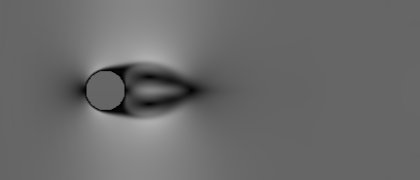
\includegraphics[scale=\scale]{../data/lbm_images/cpu_lbm_5000.png}
		\label{fig:lbm_5000}
	}
	\subfigure[10000 itérations]{%
		\centering
		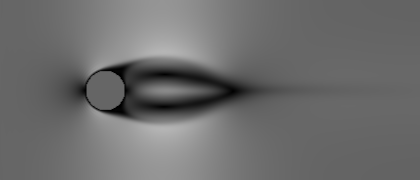
\includegraphics[scale=\scale]{../data/lbm_images/cpu_lbm_10000.png}
		\label{fig:lbm_10000}
	}
	\subfigure[15000 itérations]{%
		\centering
		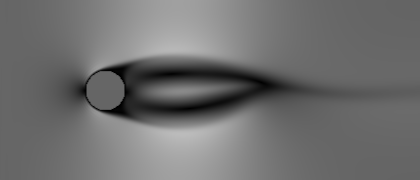
\includegraphics[scale=\scale]{../data/lbm_images/cpu_lbm_15000.png}
		\label{fig:lbm_15000}
	}
	\subfigure[20000 itérations]{%
		\centering
		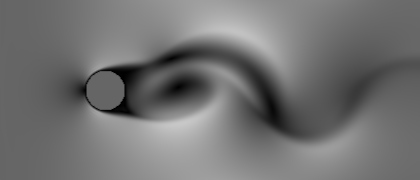
\includegraphics[scale=\scale]{../data/lbm_images/cpu_lbm_20000.png}
		\label{fig:lbm_20000}
	}
	\subfigure[25792 itérations]{%
		\centering
		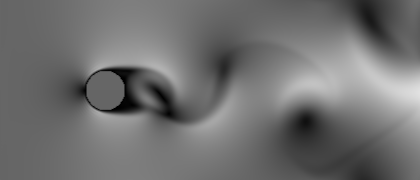
\includegraphics[scale=\scale]{../data/lbm_images/cpu_lbm_25792.png}
		\label{fig:lbm_25792}
	}
	\subfigure[39000 itérations]{%
		\centering
		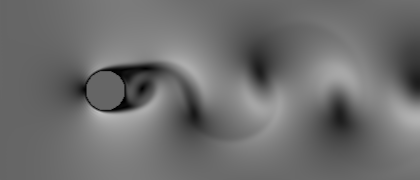
\includegraphics[scale=\scale]{../data/lbm_images/cpu_lbm_39000.png}
		\label{fig:lbm_39000}
	}
	\subfigure[40000 itérations]{%
		\centering
		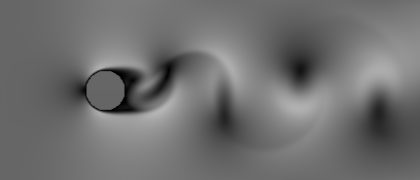
\includegraphics[scale=\scale]{../data/lbm_images/cpu_lbm_40000.png}
		\label{fig:lbm_40000}
	}
	\subfigure[41000 itérations]{%
		\centering
		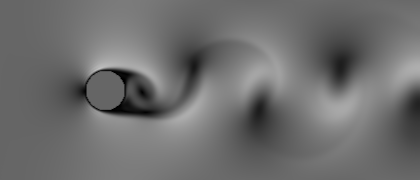
\includegraphics[scale=\scale]{../data/lbm_images/cpu_lbm_41000.png}
		\label{fig:lbm_41000}
	}
	\subfigure[42000 itérations]{%
		\centering
		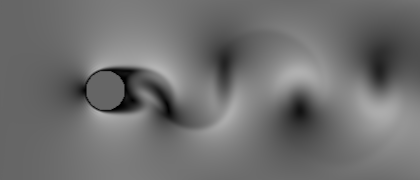
\includegraphics[scale=\scale]{../data/lbm_images/cpu_lbm_42000.png}
		\label{fig:lbm_42000}
	}
	\subfigure[43000 itérations]{%
		\centering
		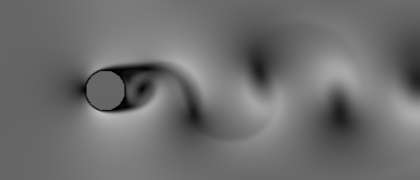
\includegraphics[scale=\scale]{../data/lbm_images/cpu_lbm_43000.png}
		\label{fig:lbm_43000}
	}
	\caption{Simulation \ac{LBM} d'un fluide autour d'un cylindre}
	\label{fig:lbm_5000_to_43000}
\end{figure}

\begin{figure}[h]
	\newcommand{\lbmsimplescale}{0.4}
	\centering
	\subfigure[100 itérations]{%
		\centering
		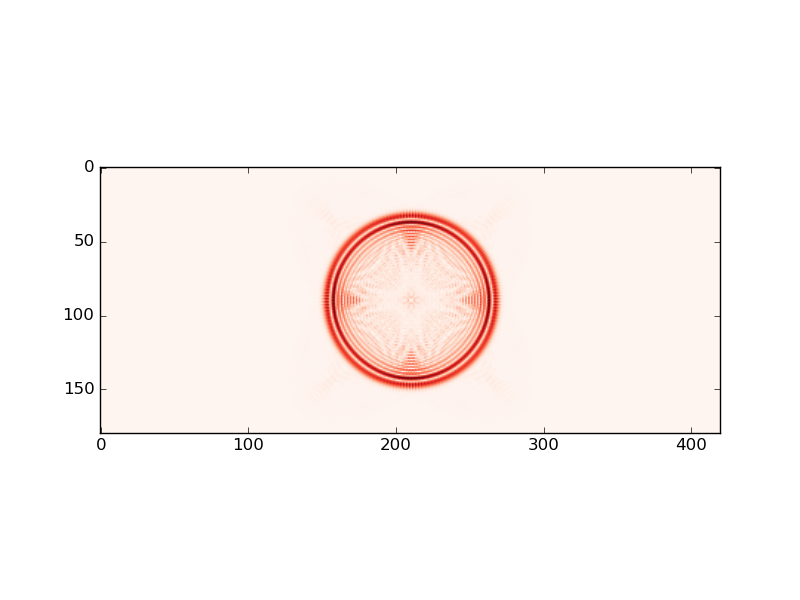
\includegraphics[scale=\lbmsimplescale, trim=45 90 50 90, clip]{images/lbm_simple/lbm_100.png}
		\label{fig:lbm_simple_100}
	}
	\subfigure[300 itérations]{%
	\centering
	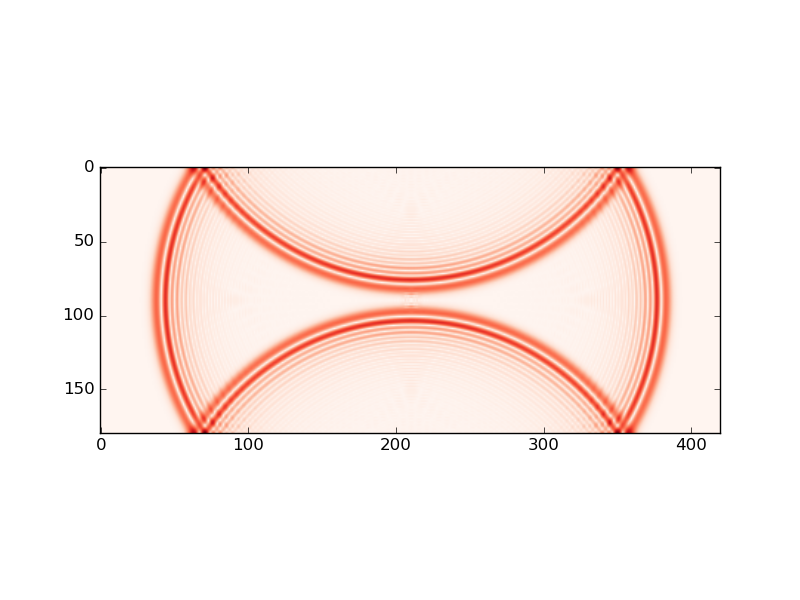
\includegraphics[scale=\lbmsimplescale, trim=45 90 50 90, clip]{images/lbm_simple/lbm_300.png}
	\label{fig:lbm_simple_300}
    }
	\subfigure[500 itérations]{%
		\centering
		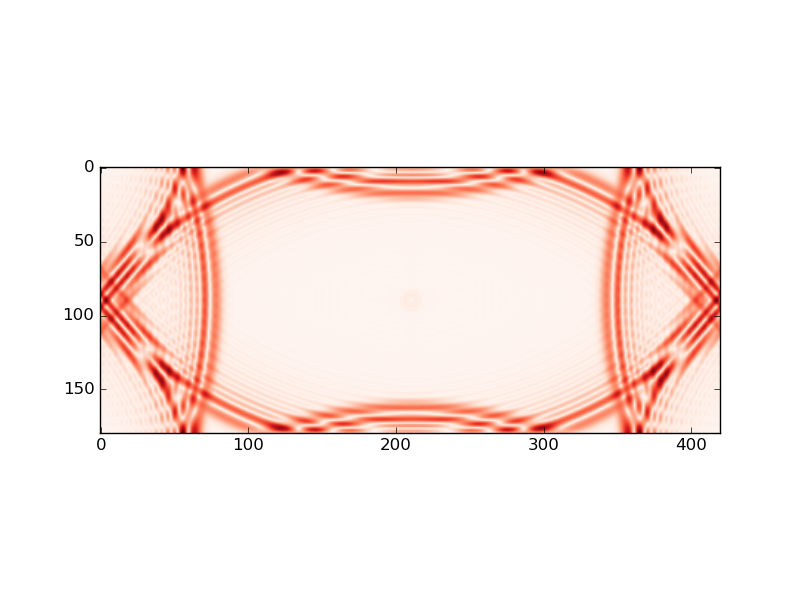
\includegraphics[scale=\lbmsimplescale, trim=45 90 50 90, clip]{images/lbm_simple/lbm_500.png}
		\label{fig:lbm_simple_500}
	}
	\subfigure[1000 itérations]{%
		\centering
		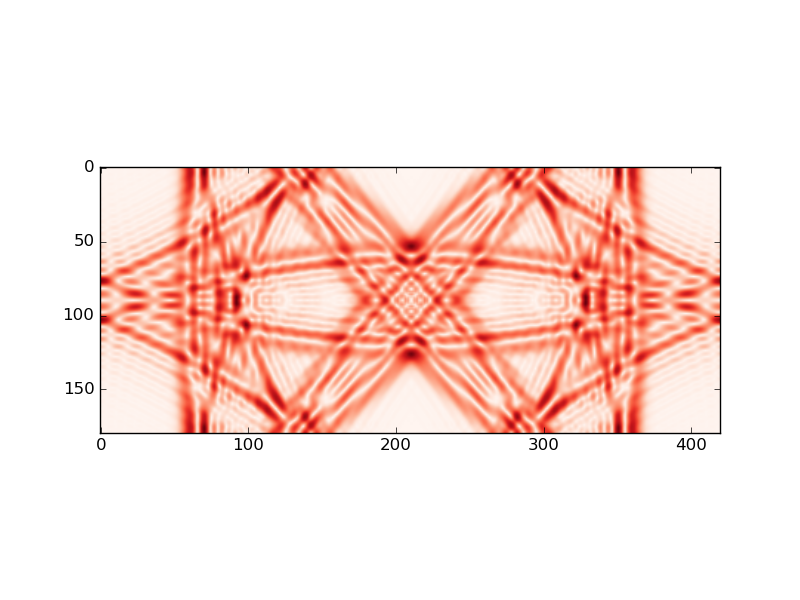
\includegraphics[scale=\lbmsimplescale, trim=45 90 50 90, clip]{images/lbm_simple/lbm_1000.png}
		\label{fig:lbm_simple_1000}
	}
	\caption{Simulation \ac{LBM} simplifiée avec une perturbation au centre du domaine}
	\label{fig:lbm_simple}
\end{figure}

\begin{figure}[h]
	\newcommand{\lbmsimplescale}{0.25}
	\centering
	\subfigure[20 itérations]{%
		\centering
		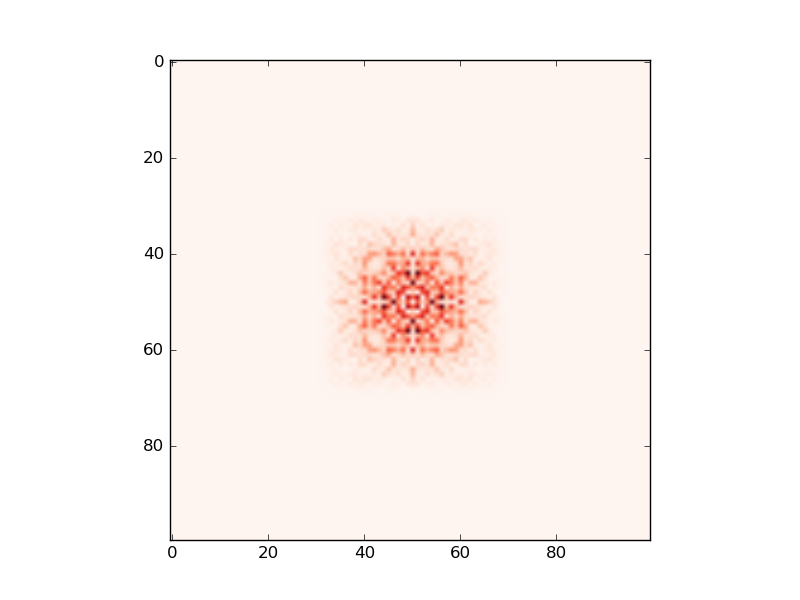
\includegraphics[scale=\lbmsimplescale, trim=103 20 105 40, clip]{images/lbm_simple_3d/lbm_20.png}
		\label{fig:lbm_simple_3d_20}
	}
	\subfigure[60 itérations]{%
		\centering
		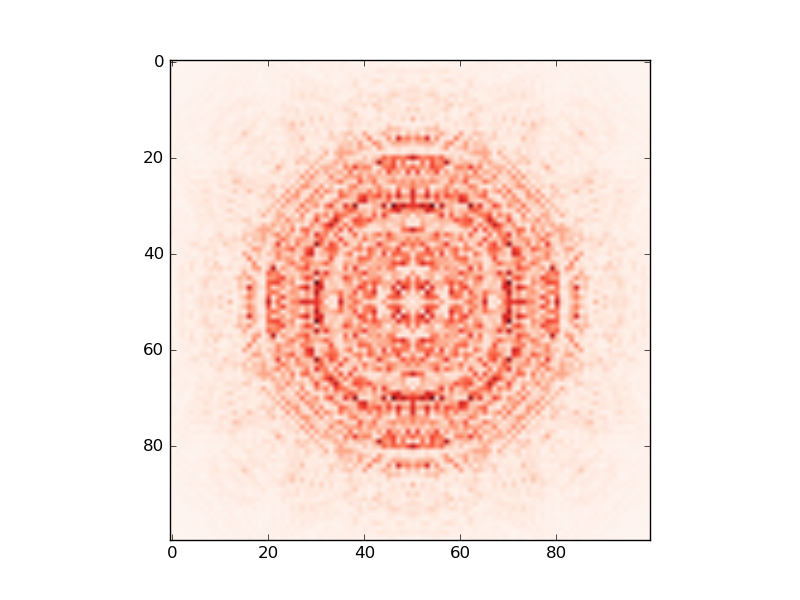
\includegraphics[scale=\lbmsimplescale, trim=103 20 105 40, clip]{images/lbm_simple_3d/lbm_60.png}
		\label{fig:lbm_simple_3d_60}
	}
	\subfigure[100 itérations]{%
		\centering
		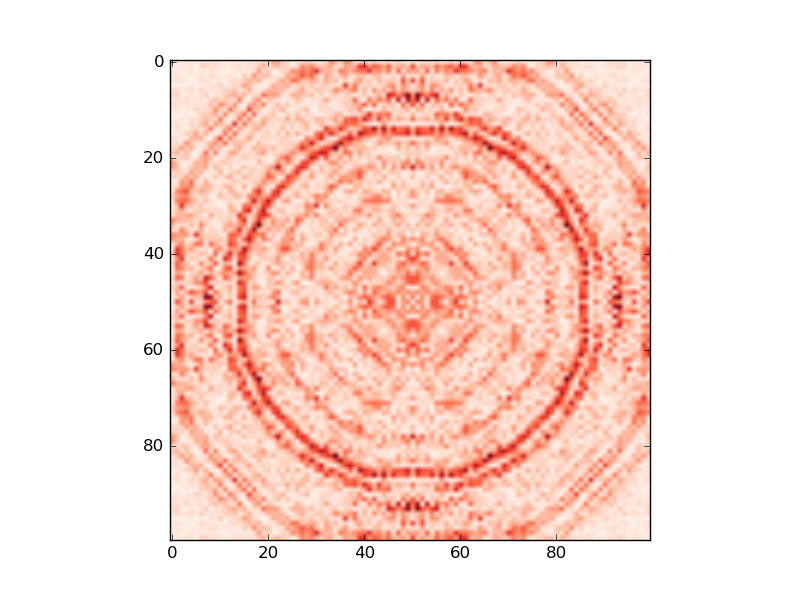
\includegraphics[scale=\lbmsimplescale, trim=103 20 105 40, clip]{images/lbm_simple_3d/lbm_100.png}
		\label{fig:lbm_simple_3d_100}
	}
	\subfigure[140 itérations]{%
		\centering
		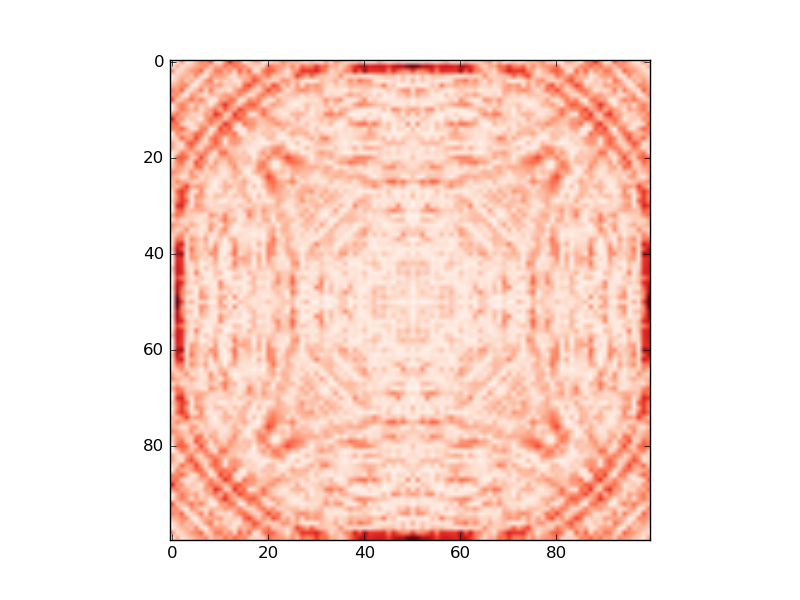
\includegraphics[scale=\lbmsimplescale, trim=103 20 105 40, clip]{images/lbm_simple_3d/lbm_140.png}
		\label{fig:lbm_simple_3d_140}
	}
	\subfigure[180 itérations]{%
		\centering
		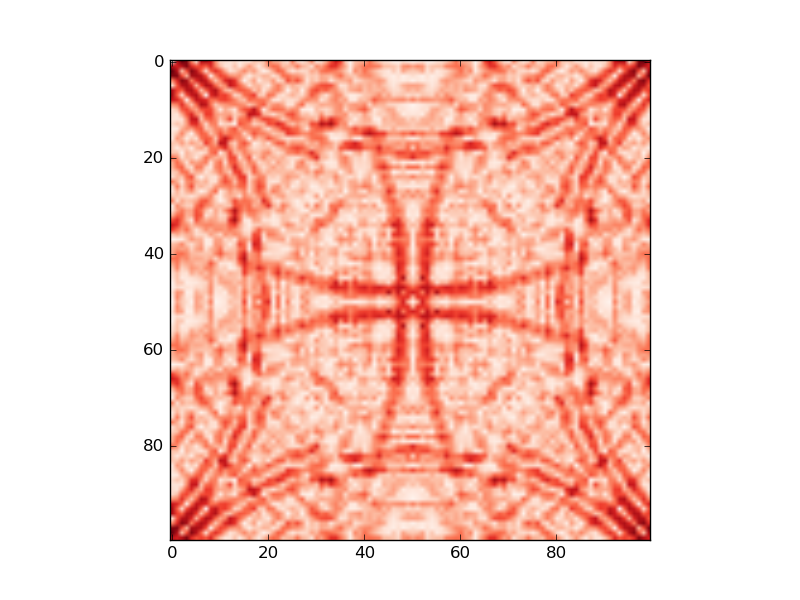
\includegraphics[scale=\lbmsimplescale, trim=103 20 105 40, clip]{images/lbm_simple_3d/lbm_180.png}
		\label{fig:lbm_simple_3d_180}
	}
	\subfigure[220 itérations]{%
		\centering
		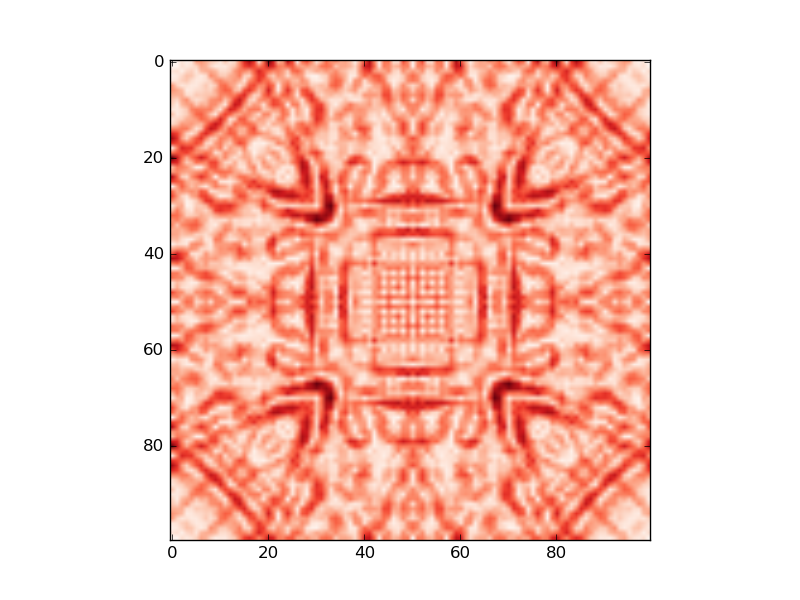
\includegraphics[scale=\lbmsimplescale, trim=103 20 105 40, clip]{images/lbm_simple_3d/lbm_220.png}
		\label{fig:lbm_simple_3d_220}
	}
	\subfigure[260 itérations]{%
		\centering
		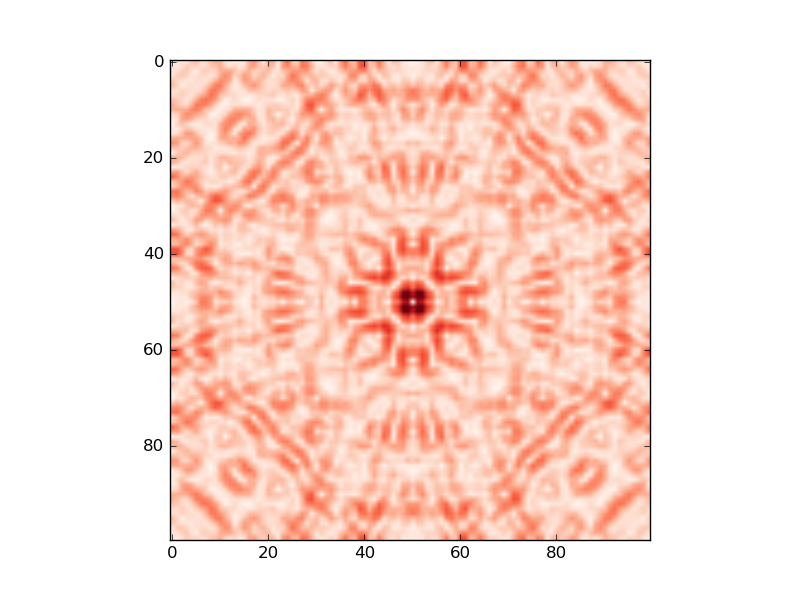
\includegraphics[scale=\lbmsimplescale, trim=103 20 105 40, clip]{images/lbm_simple_3d/lbm_260.png}
		\label{fig:lbm_simple_3d_260}
	}
	\subfigure[300 itérations]{%
		\centering
		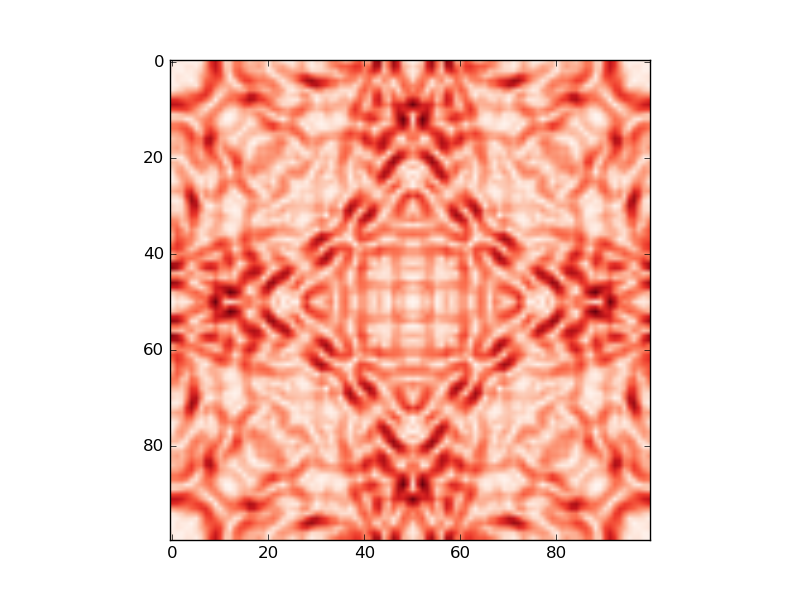
\includegraphics[scale=\lbmsimplescale, trim=103 20 105 40, clip]{images/lbm_simple_3d/lbm_300.png}
		\label{fig:lbm_simple_3d_300}
	}
	\subfigure[340 itérations]{%
		\centering
		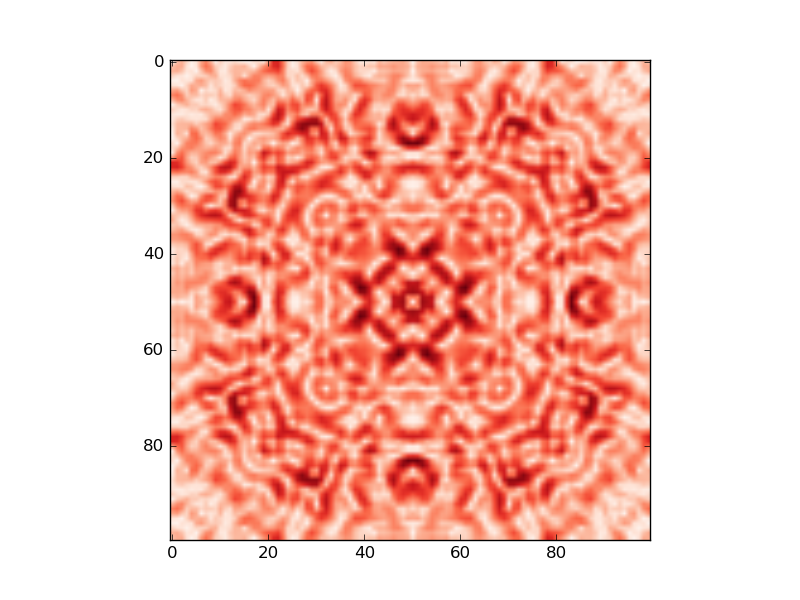
\includegraphics[scale=\lbmsimplescale, trim=103 20 105 40, clip]{images/lbm_simple_3d/lbm_340.png}
		\label{fig:lbm_simple_3d_340}
	}
	\subfigure[380 itérations]{%
		\centering
		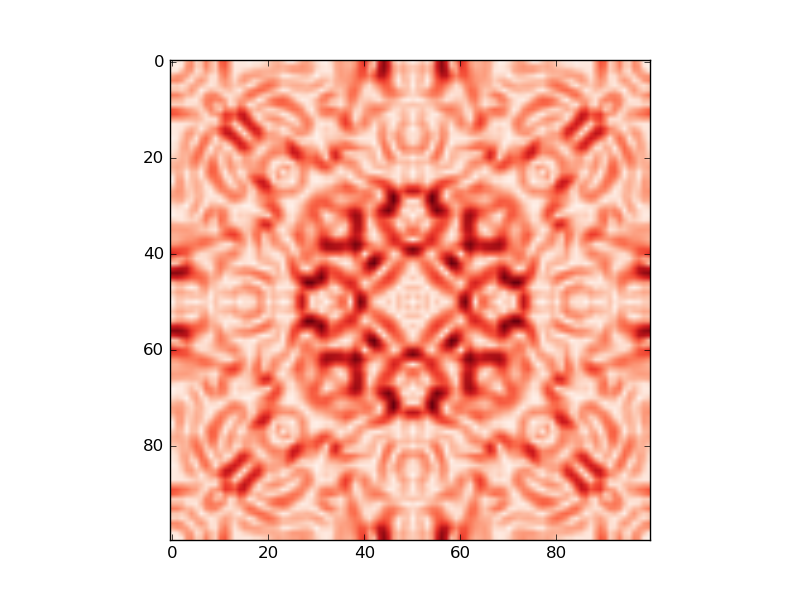
\includegraphics[scale=\lbmsimplescale, trim=103 20 105 40, clip]{images/lbm_simple_3d/lbm_380.png}
		\label{fig:lbm_simple_3d_380}
	}
	\subfigure[420 itérations]{%
		\centering
		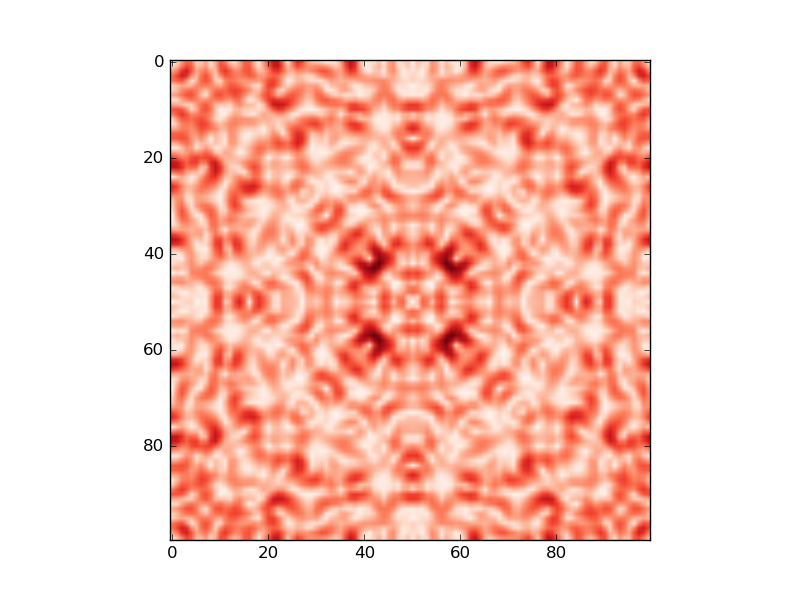
\includegraphics[scale=\lbmsimplescale, trim=103 20 105 40, clip]{images/lbm_simple_3d/lbm_420.png}
		\label{fig:lbm_simple_3d_420}
	}	
	\subfigure[460 itérations]{%
		\centering
		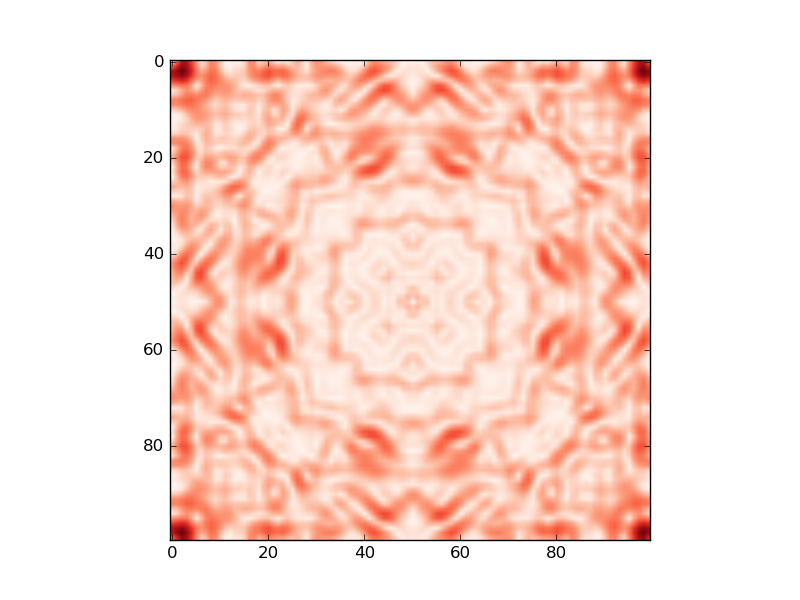
\includegraphics[scale=\lbmsimplescale, trim=103 20 105 40, clip]{images/lbm_simple_3d/lbm_460.png}
		\label{fig:lbm_simple_3d_460}
	}
	\caption{Coupe au centre d'une simulation \ac{LBM} simplifiée en 3D}
	\label{fig:lbm_simple_3d}
\end{figure}
\clearpage

\section{Implémentations Cuda}
\subsection{Sources Cuda de Sailfish}
%\subsubsection{Sources Python et extraction du code Cuda}
Sailfish est un outil de simulation de dynamiques des fluides basés sur \ac{LBM} . Bien qu'il soit écrit en Python, Sailfish génère, compile et exécute un code Cuda pour optimiser l'exécution de ses simulations sur \acs{GPU}.

Dans leur article, \citet{januszewski_sailfish_2014} décrivent son fonctionnement général, mais afin d'avoir un aperçu plus concret, une analyse du code est nécessaire. 

Une brève analyse du code Python permet d'identifier que la fonction \texttt{get\_code} génère le code Cuda. Celle-ci est appelée dans le corps de la fonction \texttt{\_update\_compute\_code} du fichier \texttt{sailfish/subdomain\_runner.py} du projet, qui compile ensuite le code généré. À l'aide d'un \acs{IDE} comme PyCharm et d'un point d'arrêt, il est alors possible d'extraire le code Cuda au format \acs{ASCII} avant qu'il soit compilé en langage machine.

Le code Cuda, plus long et plus compliqué qu'escompté, déclare de nombreuses fonctions dont plusieurs semblent avoir une utilité identique. Il est difficile d'identifier quelle portion du code est utilisé, et de quelle façon sans une analyse approfondie du fonctionnement de Sailfish.

Il n'a pas conséquent pas été particulièrement exploité.

\subsection{Code \eg{historique} de Sailfish}
Le projet disponible sur le dépôt Github de Sailfish offre une intéressante implémentation, dans le dossier \texttt{/historical}. Ces sources ne font pas partie du reste du projet, mais implémentent de façon simple une simulation D2Q9 avec \acs{LBM} sur \acs{GPU} et produit des performances respectables. On y observe les pratiques détaillées dans les sous-section qui suivent.

%\begin{itemize}
%\item \textbf{Utilisation des registres}: 
\subsubsection{Utilisation des registres}
Les populations sont conservées dans la mémoire globale, à disposition de tous les cœurs du \acs{GPU} ainsi que du \acs{CPU} à travers un \texttt{cudaMemcpy}. Toutefois, le temps d'accès à ce type de mémoire est très lent. Plutôt que d'accéder aux populations sur la mémoire globale lors de chaque calcul, celles-ci sont copiées dans des variables locales du \textit{kernel}. Ces variables, qui se situent dans les registres du \acs{GPU}, le type de mémoire le plus rapide, sont alors utilisées dans les calculs et sont finalement copiées dans la mémoire globale à la fin du \textit{kernel}.
Cette méthode réduit sensiblement le nombre d'accès à la mémoire globale et augmente ainsi nettement les performances.
%\item \textbf{Structure de donnée des populations}:
\subsubsection{Structure de donnée des populations}
Les populations sont conservées dans 9 tableaux différent, soit un par direction, de la taille du domaine. L'arrangement mémoire suit par conséquent le modèle \acs{SoA}.

%\item \textbf{Calcul des populations}: 
\subsubsection{Calcul des populations}
Plutôt qu'utiliser une boucle pour itérer sur les différentes directions et en calculer de façon générique leur état (comme l'equilibrium), celles-ci sont dépliées pour effectuer un à un le calcul adéquat.

%\item \textbf{Streaming sur la mémoire partagée (coalescing)}: 
\subsubsection{\textit{Streaming coalesced}}\label{title-streaming-coalesced}
Le \textit{streaming} copie les directions de la population calculée par un cœur \acs{GPU} dans les populations adjacentes qui résident en mémoire globale. L'accès à cette mémoire est lent, mais peut être optimisé par des accès contigus et aligné sur 16 octets. On dit de ce schéma d'accès à la mémoire qu'il est \eg{\textit{coalesced}}.

Les \textit{threads} au sein d'un bloc sont activés par \textit{warp} de 32 sur l'axe des \textit{x}. Ces \textit{threads}, qui accèdent à la mémoire globale lors du \textit{streaming}, doivent chacun y écrire une à une les valeurs des directions calculées qui résident dans leurs registres, soit 32 doubles par direction. La mémoire globale est accédée par transaction de 32, 64, 128 ou 256 octets. Par conséquent, si les directions des 32 populations (qui occupent 256 octets) accédées par les \textit{threads} sont contiguës en mémoires, seule une transaction en mémoire globale est nécessaire. 

Les figures~\ref{fig:sailfish_hist_misaligned} à~\ref{fig:sailfish_hist_dir_aligned} illustrent le \textit{streaming} d'un bloc de 4 \textit{threads} sur un domaine $12 \times 3$.
Sur la figure~\ref{fig:sailfish_hist_misaligned}, les \textit{threads} utilisent un schéma d'accès où les directions sont propagées aux populations adjacentes directement en mémoire globale. L'arrangement en mémoire des directions sur les populations accédées est illustré par la figure~\ref{fig:sailfish_hist_alignment}. On observe sur la figure~\ref{fig:sailfish_hist_dir_misaligned} que l'écriture des valeurs pour les directions nord et sud est naturellement alignée. Ce n'est toutefois pas le cas pour les autres directions puisqu'elles impliquent un décalage en $x$ de $-1$ à l'est et $+1$ à l'ouest. Leur accès n'est par conséquent pas \textit{coalesced}.

\begin{figure}[H]
	\centering
%	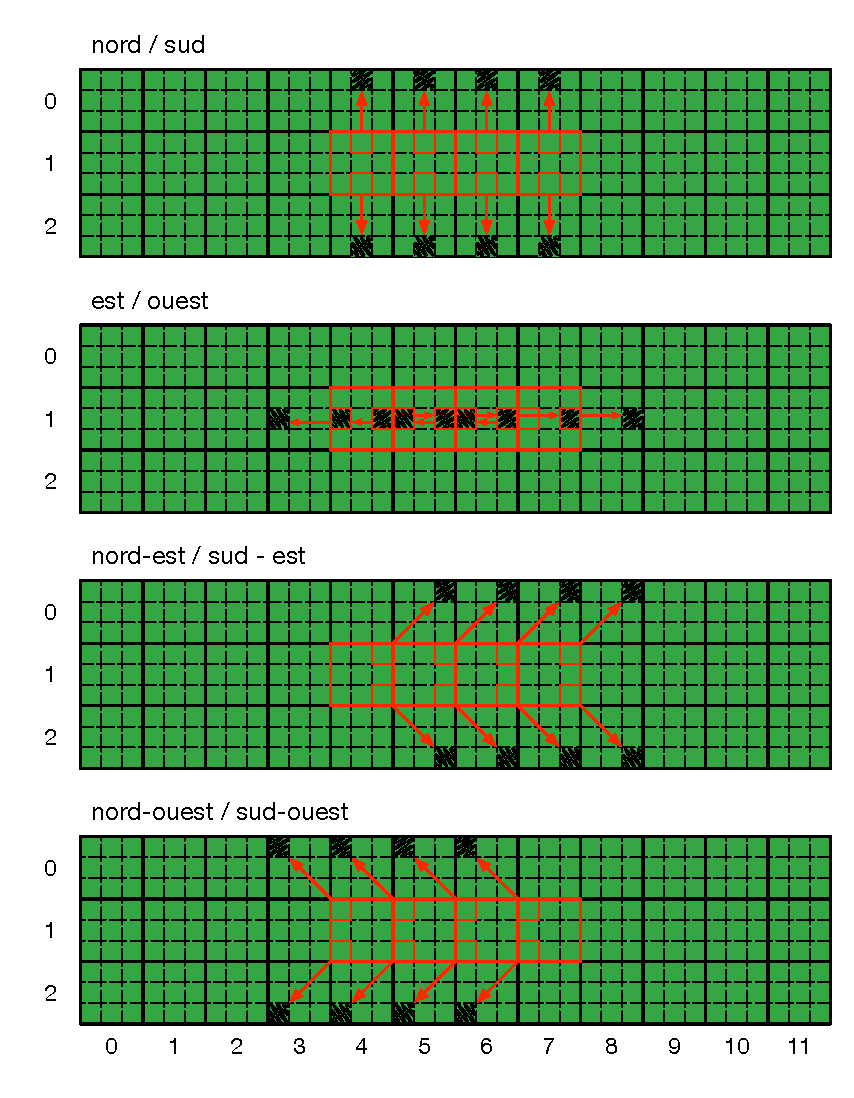
\includegraphics[fbox,scale=1.05]{images/streaming/sailfish_hist_misaligned.pdf}
	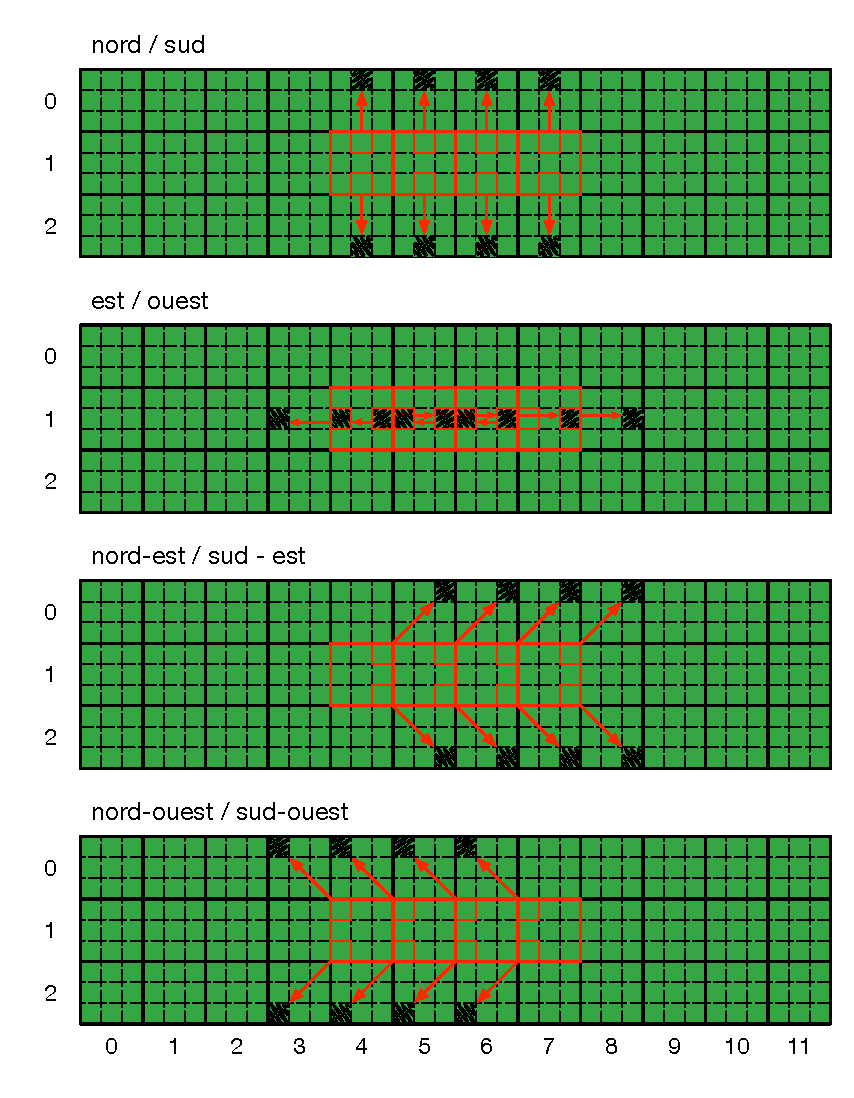
\includegraphics[fbox,scale=.7]{images/streaming/sailfish_hist_misaligned.pdf}
	\caption{\textit{Streaming} \textit{uncoalesced} d'un bloc de quatre \textit{threads}}
	\label{fig:sailfish_hist_misaligned}
\end{figure}

\begin{figure}[H]
	\centering
	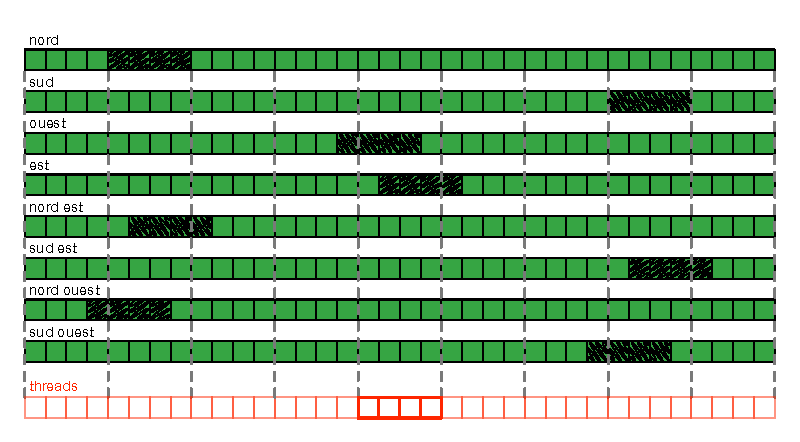
\includegraphics[fbox,scale=1]{images/streaming/sailfish_hist_alignment.pdf}
	\caption{Arrangement en mémoire des populations du \textit{streaming} de la figure~\ref{fig:sailfish_hist_misaligned}}
	\label{fig:sailfish_hist_alignment}
\end{figure}

\begin{figure}[H]
	\centering
	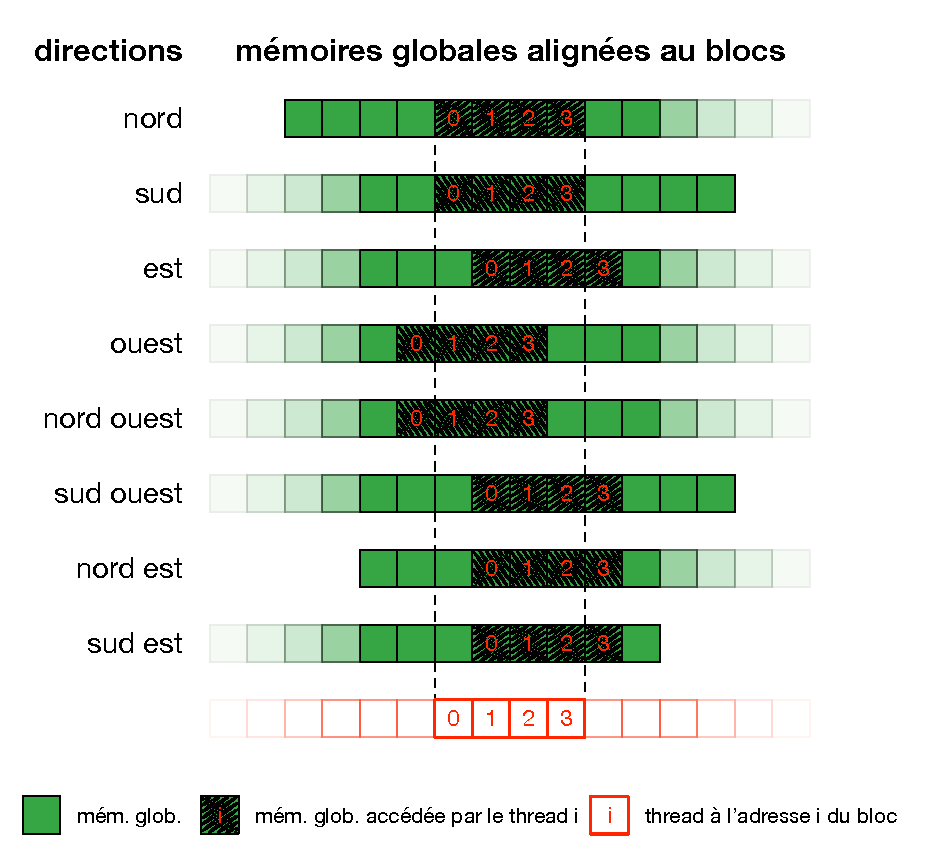
\includegraphics[fbox,scale=0.95]{images/streaming/sailfish_hist_dir_misaligned.pdf}
	\caption{Accès mémoire désaligné des \textit{threads} lors du \textit{streaming} de la figure~\ref{fig:sailfish_hist_misaligned}}
	\label{fig:sailfish_hist_dir_misaligned}
\end{figure}

\begin{figure}[H]
	\centering
	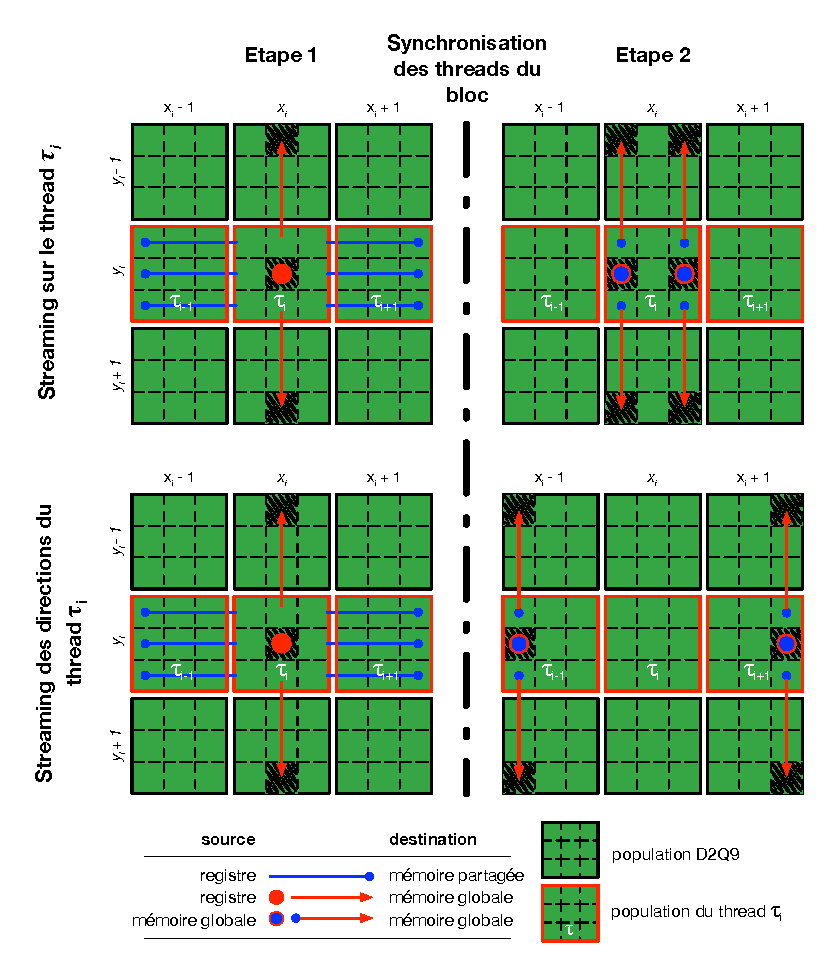
\includegraphics[fbox,scale=1.1]{images/streaming/sailfish_hist_ti.pdf}
	\caption{Stratégie de \textit{streaming} \textit{coalesced} par réalignement des populations en mémoire partagée}
	\label{fig:sailfish_hist_ti}
\end{figure}
\pagebreak

Pour remédier au désalignement inhérent à la position de la population calculée par chaque \textit{thread}, une stratégie en deux étapes est utilisée pour écrire les directions en mémoire globale (figure~\ref{fig:sailfish_hist_ti}). 
\begin{enumerate}
\item Dans un premier temps, au lieu de les propager directement en mémoire globale, les directions nord-ouest, ouest et sud-ouest de chaque \textit{thread} au sein d'un bloc sont écrites en mémoire partagée sur l'indice du \textit{thread} de gauche ($x-1$) et les directions nord-est, est et sud-est sur l'indice du \textit{thread} de droite ($x+1$).
\item Dans un second temps, chaque \textit{thread} cherche en mémoire partagée es directions inscrites à son indice et les propage en mémoire globale aux populations en dessus ($x - N_x$) et en dessous ($x + N_z$).
\end{enumerate}
Une barrière de synchronisation entre les deux étapes assure que chaque \textit{thread} a bien calculé et inscrit les directions en mémoire partagée, à l'attention de ses voisins, avant de procéder à la seconde étape.

La figure~\ref{fig:sailfish_hist_aligned} illustre ce mécanisme exécuté simultanément sur chaque \textit{thread} d'un bloc et la figure~\ref{fig:sailfish_hist_dir_aligned} l'alignement des indices des accès en mémoire globale. On constate avec cette stratégie des accès \textit{coalesced}, à l'exception de ceux des \textit{thread} au bord du bloc. En effet, ces derniers n'ont pas accès à la mémoire partagée du \textit{thread} adjacent qui se trouve dans un bloc différent. Ils doivent par conséquent propager certaines directions directement en mémoire globale.

\begin{figure}[H]
	\centering
	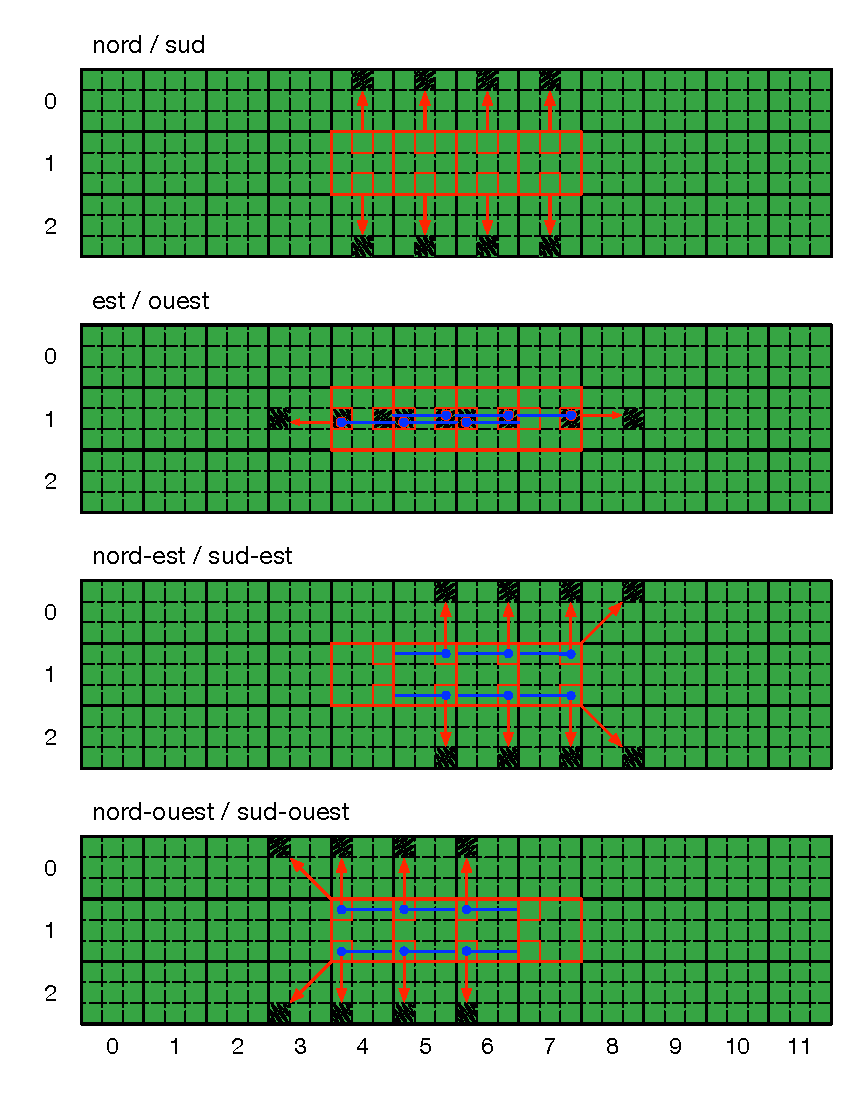
\includegraphics[fbox,scale=.7]{images/streaming/sailfish_hist_aligned.pdf}
	\caption{\textit{Streaming} \textit{coalesced} d'un bloc de quatre \textit{threads}}
	\label{fig:sailfish_hist_aligned}
\end{figure}


Les directions nord et sud, déjà alignées, sont directement propagées en mémoire globale, indépendamment lors de la première ou seconde étape.

L'exemple utilisé illustre des blocs de 4 \textit{thread} par souci de lisibilité. En pratique, ceux-ci sont plus grands (32 ou 64) afin de réduire ainsi le nombre d'accès \textit{uncoalesced}.

%\end{itemize}


\begin{figure}[H]
	\centering
	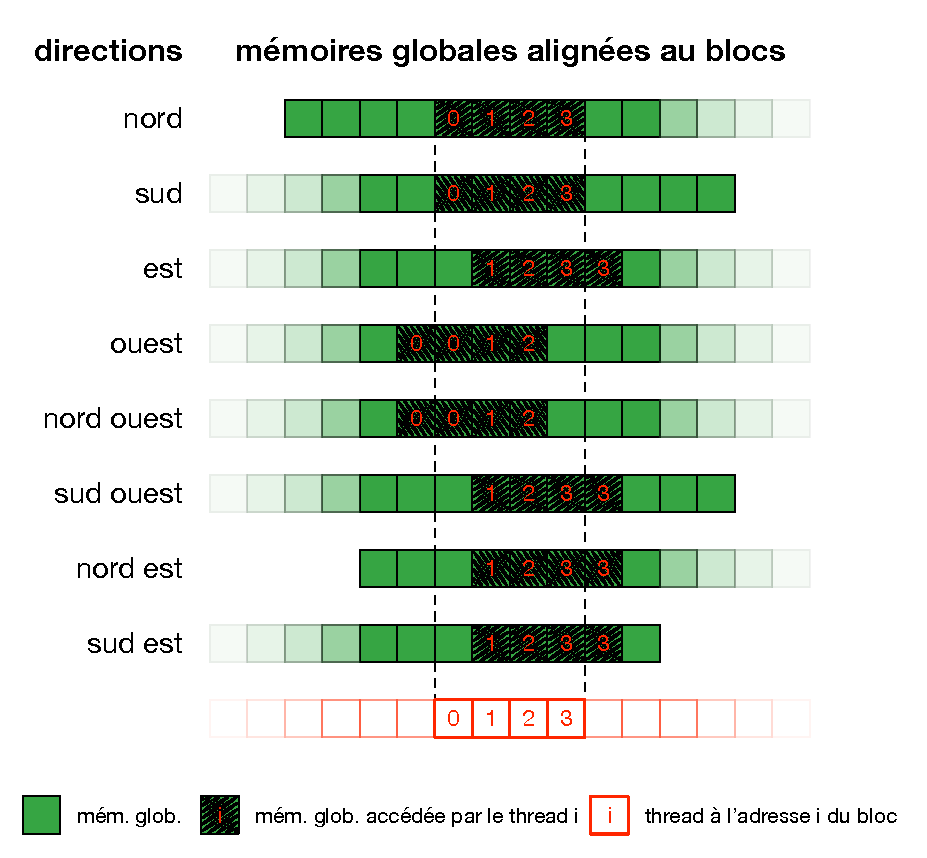
\includegraphics[fbox,scale=1]{images/streaming/sailfish_hist_dir_aligned.pdf}
	\caption{Accès mémoire aligné des \textit{threads} lors du \textit{streaming} de la figure~\ref{fig:sailfish_hist_aligned}}
	\label{fig:sailfish_hist_dir_aligned}
\end{figure}

Toutefois, \citet{obrecht_global_2011} cherchent à éviter l'usage de la mémoire partagée plutôt qu'éviter à tout prix les accès \textit{uncoalesced}. En effet, bien que cette stratégie se montre efficace sur les anciennes générations de \acs{GPU}, le gain en performance semble nettement moindre sur les plus \acs{GPU}, qui réduisent le coût des accès \textit{uncoalesced} à l'aide de la mémoire cache. 

Un certain nombre de travaux montrent que les accès \textit{uncoallesced} en lecture sont légèrement moins couteux que les accès en écriture et qu'il est plus intéressant de profiter de cette propriété que d'utiliser la mémoire partagée. En effet, les accès à cette mémoire, pour y copier puis y lire les populations, bien qu'ils soient rapides, ne sont pas gratuits pour autant.

\subsection{Différences entre calculs sur CPU et GPU} \label{title-floats}
Cuda supporte la norme IEEE 754 pour les calculs avec nombre flottants \cite{ZZZweb_cuda_2017}. Toutefois, dans la première implémentation Cuda de \acs{LBM} , le protocole de test (décrit en section~\ref{title-tests}) a montré des différences sur certains calculs réalisés par les codes \acs{CPU}.

Pour les mesurer, un code \ac{LBM} 2D \acs{CPU} et un code \acs{GPU} ont été implémentés et leurs résultats comparés. La figure~\ref{fig:lbm_float_deltas} illustre la différence moyenne entre les valeurs calculées sur \acs{CPU} et \acs{GPU} pour l'ensemble des populations $f_{in}$ de chaque itération.

\begin{figure}[H]
	\centering
	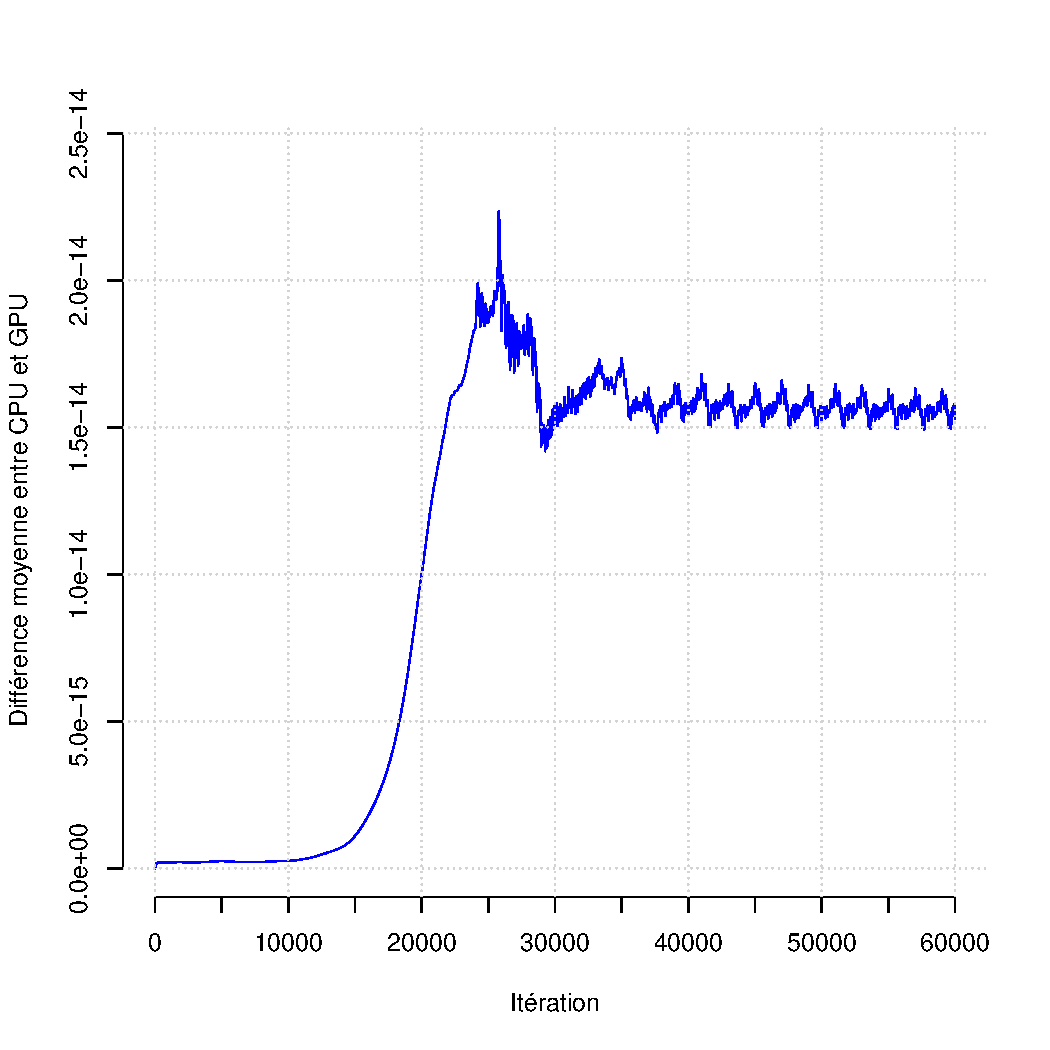
\includegraphics[scale=0.685, fbox]{../data/lbm_cpu_vs_gpu/deltas/Rplots.pdf}
	\caption{Différences moyennes (par itération) entre les calculs sur \acs{CPU} et \acs{GPU}}
	\label{fig:lbm_float_deltas}
\end{figure}

L'écart entre les résultats observés sur \acs{CPU} et \acs{GPU} suit les étapes de la simulation réalisée (fluide autour d'un cylindre) illustrée par les figures~\ref{fig:lbm_5000_to_43000}:
\begin{itemize}
	\item entre 0 et environ 12000 itérations, une trace se forme derrière le cylindre et l'écart moyen reste faible et stable (quinze zéros après la virgule);
	\item entre 15000 et 20000 itérations, la trace commence à osciller et l'écart augmente brutalement (treize zéros après la virgule);
	\item à la 25792$^{\textrm{ième}}$ itération, l'oscillation commence à se stabiliser et l'écart atteint son maximum (toujours treize chiffres après la virgule);
	\item dès environ 36000 itérations, l'oscillation est stabilisée (comme le montrent les figures~\ref{fig:lbm_39000} et~\ref{fig:lbm_43000}, le même motif réapparaît toutes les 4000 itérations environ) et les écarts avec.
\end{itemize}

Cette différence entre certains résultats sur \acs{CPU} et \acs{GPU} est le fruit d'une optimisation du compilateur Cuda. Sur \acs{CPU}, lorsqu'une opération du type $r = x \times y+z$ est rencontrée, le processeur calcul d'abord $r_{xy} = x \times y$ puis $r = r_{xy} + z$. Deux opérations sont donc réalisées, ce qui implique deux potentiels arrondis dans le cas des nombres flottants. Sur \acs{GPU}, le compilateur optimise ce type de calculs \cite{ZZZweb_cuda_2017-1} avec la fonction \ac{FMA} qui réalise $x \times y+z$ en une seule opération. Le calcul est ainsi plus rapide et précis (puisqu'un seul arrondi est effectué).

Comme le souligne la documentation de Cuda, cette optimisation n'est pas forcément souhaitable dans certaines circonstances et peut être évitée avec l'utilisation de fonctions intrinsèques \cite{ZZZweb_cuda_2017-1, ZZZweb_cuda_2017-2}.

Cette précaution force le \acs{GPU} à effectuer les multiplications et additions indépendamment et permet de s’assurer que les calculs réalisés sur \acs{CPU} et \acs{GPU} produisent les mêmes résultats.

\subsection{Passage de la 2D à la 3D et bibliothèque \texttt{lbmcuda}}
De nombreuses implémentations 2D ont été réalisées. Elles ont d’abord été adaptées des portages en C, puis inspirées par le code historique de Sailfish, jusqu’à la dernière (nommé \texttt{lbm\_opt2}) qui a fini par atteindre des performances acceptables (450 MLUPS sur une Nvidia GeForce GT 750M). 

Pour passer du modèle D2Q9 à D3Q19, les 10 populations manquantes sont ajoutées en mémoire globale et sont intégrées aux calculs de la collision ainsi qu'au \textit{streaming}. À ce stade, l'implémentation utilisait encore la mémoire partagée pour le \textit{streaming}. Suite à l'ajout des populations, l'implémentation est testée avec et sans ce mécanisme. Mais comme l'évoque la section~\ref{title-streaming-coalesced}, il s'avère que les \textit{GPU} récents ne pâtissent pas autant des accès \textit{uncoalesced} en raison d'optimisation automatique à travers l'utilisation de la mémoire cache.

D'autres optimisations, proposées par \citet{januszewski_sailfish_2014} et \citet{tran_performance_2017} améliorent les performances:
\begin{itemize}
\item \textbf{Registres}: Les registres sont utilisés par certaines variables locales du \textit{kernel}. C'est le type de mémoire le plus rapide, mais leur nombre est restreint. En dépasser la limite entraîne un débordement en mémoire local, moins rapide, et par conséquent une perte de performance. Hélas, le passage de D2Q9 à D3Q19 augmente significativement le nombre de variables locales et par conséquent l'utilisation des registres. Ne pas précalculer des valeurs utilisées plusieurs fois, et qui devraient être ainsi stockées dans des variables intermédiaires, mais les recalculer à chaque fois semble être une \eg{optimisation} contre-intuitive, mais réduit le nombre de registres et par conséquent contribue à améliorer les performances.
\item \textbf{Cache L1}: \citet{januszewski_sailfish_2014} relèvent que les accès à la mémoire locale dus aux dépassements du nombre de registres passent par la cache L1 et que plus sa part inutilisée est grande et moins la mémoire globale est mise à contribution. Ils proposent ainsi d'augmenter la taille de la cache et de désactiver la cache L1 pour les accès à la mémoire globale. La première opération est accomplie par \texttt{cudaDeviceSetCacheConfig}:
\begin{lstlisting}[numbers=none]
if ( cudaDeviceSetCacheConfig (cudaFuncCachePreferL1) != cudaSuccess)
	fprintf(stderr, "cudaFuncSetCacheConfig failed\n");
\end{lstlisting}
et la seconde en compilant le code Cuda avec les arguments \texttt{-Xptxas -dlcm=cg}.
\item \textbf{Divisions par des multiplications}: Les multiplications sont un peu plus rapides que les divisions. Remplacer une division par une multiplication, lorsque cela est possible, peut ainsi améliorer les performances. Si plusieurs calculs requièrent une division par la même valeur (comme avec \textit{rho} dans la fonction \textit{macroscopic}), l'inverse de sa valeur peut être calculé initialement puis être multiplié par la suite pour éviter plusieurs divisions. Cette méthode a toutefois l'inconvénient de modifier parfois très légèrement le résultat du calcul en raison d'un arrondi différent avec les valeurs flottantes et ajoute une variable locale intermédiaire.
\end{itemize}

Finalement, en vue de son intégration à Palabos et afin d'en simplifier l'utilisation, l'implémentation Cuda est portée dans une bibliothèque dynamique nommée \texttt{lbmcuda} que le projet \texttt{lbm\_simple\_lbmcuda} utilise pour implémenter la même configuration que \texttt{lbm\_simple} en C et Python. La bibliothèque implémente les principales fonctions suivantes:

\begin{itemize}
\item \texttt{lbm\_simulation\_create}: Création d'un domaine de simulation en spécifiant ses dimensions ainsi que la valeur d'omega.
\item \texttt{lbm\_simulation\_update}: Mets à jour les populations du domaine sur une itération.
\item \texttt{lbm\_lattices\_read} et \texttt{lbm\_lattices\_read}: Transfert de l'intégralité des populations du domaine respectivement depuis et vers le \acs{GPU}.
\item \texttt{lbm\_lattices\_read\_subdomain} et \texttt{lbm\_lattices\_write\_subdomain}: Transfert partiel du domaine.
\item \texttt{lbm\_read\_palabos\_subdomain} et \texttt{lbm\_write\_palabos\_subdomain} : Transfert partiel du domaine avec réorganisation mémoire selon l'ordre utilisé par Palabos (voir section~\ref{title-strategie_reorganisation}).
\end{itemize}

\section{Intégration à Palabos}
\subsection{Co-processeurs}
\subsubsection{Fonctionnement}
Il est possible de demander à Palabos de découper un domaine de recherche en plusieurs sous-domaines afin de les calculer indépendamment les uns des autres. Comme l'illustre la figure~\ref{fig:plb_domain_split}, un sous-domaine possède une portion unique du domaine de recherche (vert) ainsi qu'une marge extérieure (bleu) qui s'entrelace avec les zones centrales des sous-domaines adjacents. Son rôle est de propager les valeurs calculées par les sous-domaines voisins pour calculer la zone centrale (verte).

\begin{figure}[h]
	\centering
	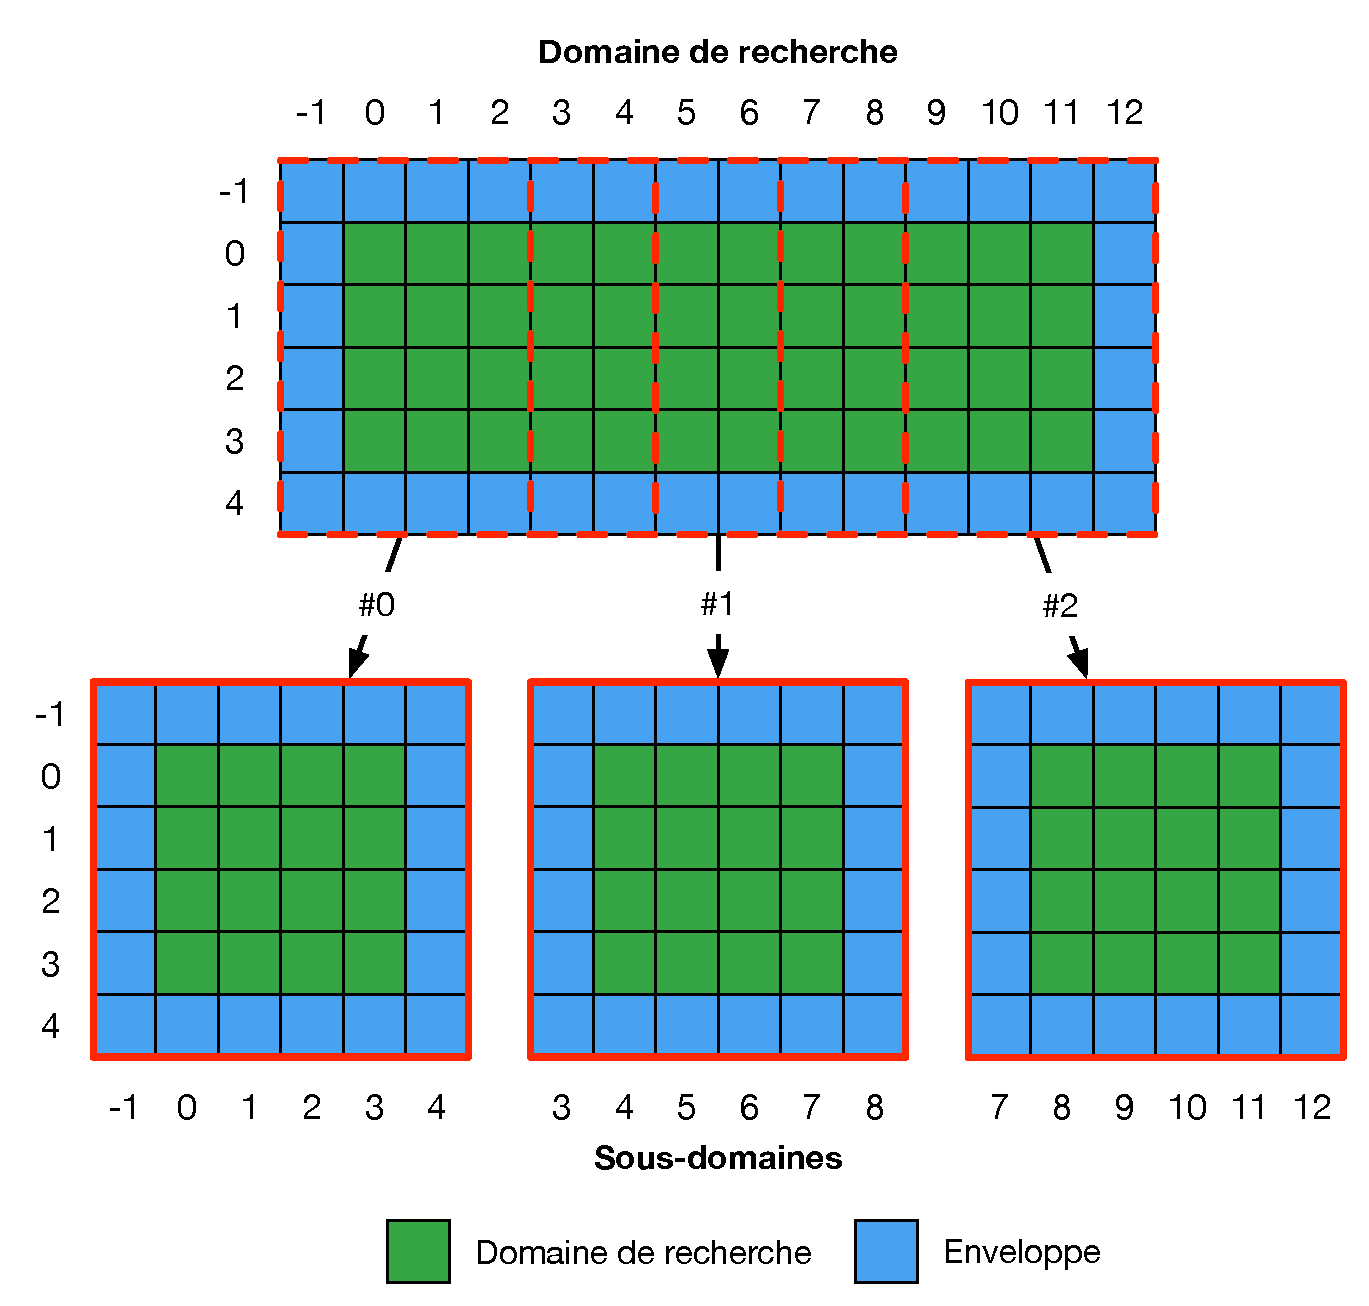
\includegraphics[scale=0.65, fbox]{images/decoupage_domaine_palabos.pdf}
	\caption{Découpage d'un domaine 12x4 en trois sous-domaines par Palabos}
	\label{fig:plb_domain_split}
\end{figure}

Ce découpage permet
\begin{enumerate*}
\item de distribuer la simulation sur différents nœuds (à l'aide d'\acs{MPI}) et
\item de déléguer les calculs à un \ac{CP} spécialisé.
\end{enumerate*}

Un \ac{CP} (ou accélérateur) est un module capable de calculer l'état d'un sous-domaine, normalement pris en charge par Palabos sur \acs{CPU}, mais cette fois confié par celui-ci. Son objectif est d'accélérer la vitesse des calculs en se spécialisant sur un certain type de sous-domaine. L'utilisation d'un \ac{CP} est illustrée dans le programme d'exemple \texttt{coProcessor}\footnote{dossier: \texttt{<palabos root>/examples/codesByTopic/coProcessor}} fourni dans Palabos où l'on distingue cinq étapes importantes.

\begin{enumerate}
\item \textbf{Initialisation des \ac{CP}}: On commence par assigner un \ac{CP} aux sous-domaines désignés d'un espace de recherche découpé au préalable.
\item \textbf{Transfert \acs{CPU} à \ac{CP}}: À ce stade, seul Palabos connaît l'état de l'espace de recherche. Par conséquent, on transfère les valeurs des populations dans les sous-domaines délégués aux \ac{CP}.
\item \textbf{Calcul du \ac{CS}}: On calcule \textit{une} itération avec \ac{LBM}  sur l'ensemble des sous-domaines (avec Palabos et les \ac{CP}).
\item \textbf{Transfert \ac{CP} à \acs{CPU}}: À ce stade, contrairement à la seconde étape, Palabos ignore l'état des sous-domaines assignés au \ac{CP}, que seuls eux connaissent. On transfère cette fois ces valeurs dans le sens opposé.
\item \textbf{Duplication des chevauchements}:  Les enveloppes des sous-domaines se chevauchent. Il faut par conséquent dupliquer les valeurs d'un sous-domaine, calculé à l'étape précédente, dans les enveloppes des sous-domaines voisins.
\end{enumerate}

Au terme de ce processus, une itération complète est ainsi effectuée. Pour en calculer une autre, on recommencera depuis la seconde étape. 

\subsubsection{Implémentation}
Un co-processeur n'est autre qu'une classe qui hérite de \texttt{CoProcessor3D}. Pour fonctionner, elle doit implémenter les principales méthodes suivantes. Elles sont respectivement appelées lors des quatre premières étapes mentionnées précédemment.

\begin{itemize}
\item \texttt{addDomain}: Associe un \texttt{ID} à un sous-domaine attribué au \ac{CP} et en défini les dimensions.
\item \texttt{send}: Envoie l'état du sous-domaine, de la mémoire de Palabos vers celle du \ac{CP}.
\item \texttt{collideAndStream}: Calcule une itération sur un sous-domaine du \ac{CP}.
\item \texttt{receive}: Envoie l'état du sous-domaine, de la mémoire du \ac{CP} vers celle de Palabos.
\end{itemize}

C'est ce mécanisme de \ac{CP} qui est utilisé pour donner à Palabos la capacité de calculer un sous-domaine sur \acs{GPU}.

\subsection{Transfert mémoire entre Palabos et un \acs{CP} }\label{title-transfert_palabos_cp}
À chaque itération, il est nécessaire de transférer l'état des populations des sous-domaines deux fois:
\begin{enumerate}
\item \textbf{Avant de calculer les populations des \ac{CP}}: depuis Palabos vers les \ac{CP}, pour propager les populations calculées par les sous-domaines adjacents.
\item \textbf{Après les avoir calculés sur les \ac{CP}}: depuis les \ac{CP} vers Palabos, pour propager leurs populations à l'itération suivante.
\end{enumerate}

Lors de l'appel à méthode \texttt{send} et \texttt{receive}, Palabos transmet un espace mémoire contigu où les populations sont respectivement écrites et lues. Il est adressé en calculant l'index suivant:
\begin{equation}
i_{pal} = ( x*N_z*N_y + y*N_z + z) * 19 + dir
\end{equation}
avec la dimension  $N_y$ et $N_z$ du sous-domaine en $y$ et $z$ et $i_{pal}$ l'index de la population en $\{x,y,z\}$ avec pour direction $dir$ (figure~\ref{fig:plb_population_index}):

\noindent\begin{minipage}{.25\linewidth}
\begin{align*}
&dir_{center} &=  0 \\
&dir_{west} &=  1 \\
&dir_{south} &=  2 \\
&dir_{center}^{bottom} &=  3 \\
&dir_{south west} &=  4
\end{align*}
\end{minipage}%
\begin{minipage}{.25\linewidth}
\begin{align*}
&dir_{north west} &=  5 \\
&dir_{west}^{bottom} &=  6 \\
&dir_{west}^{top} &=  7 \\
&dir_{south}^{bottom} &=  8 \\
&dir_{south}^{top} &=  9 
\end{align*}
\end{minipage}%
\begin{minipage}{.25\linewidth}
\begin{align*}
&dir_{east} &= 10 \\
&dir_{north} &= 11 \\
&dir_{center}^{top} &= 12 \\
&dir_{north east} &= 13 \\
&dir_{south east} &= 14 
\end{align*}
\end{minipage}
\begin{minipage}{.25\linewidth}
\begin{align*}
&dir_{east}^{top} &= 15 \\
&dir_{east}^{bottom} &= 16 \\
&dir_{north}^{top} &= 17 \\
&dir_{north}^{bottom} &= 18\\
\end{align*}
\end{minipage}\\

Si le \ac{CP} utilise la même stratégie d'adressage, une simple copie de la mémoire suffit. Dans le cas inverse, il faut considérer une étape de réorganisation de la mémoire.

\begin{figure}[h]
	\centering
	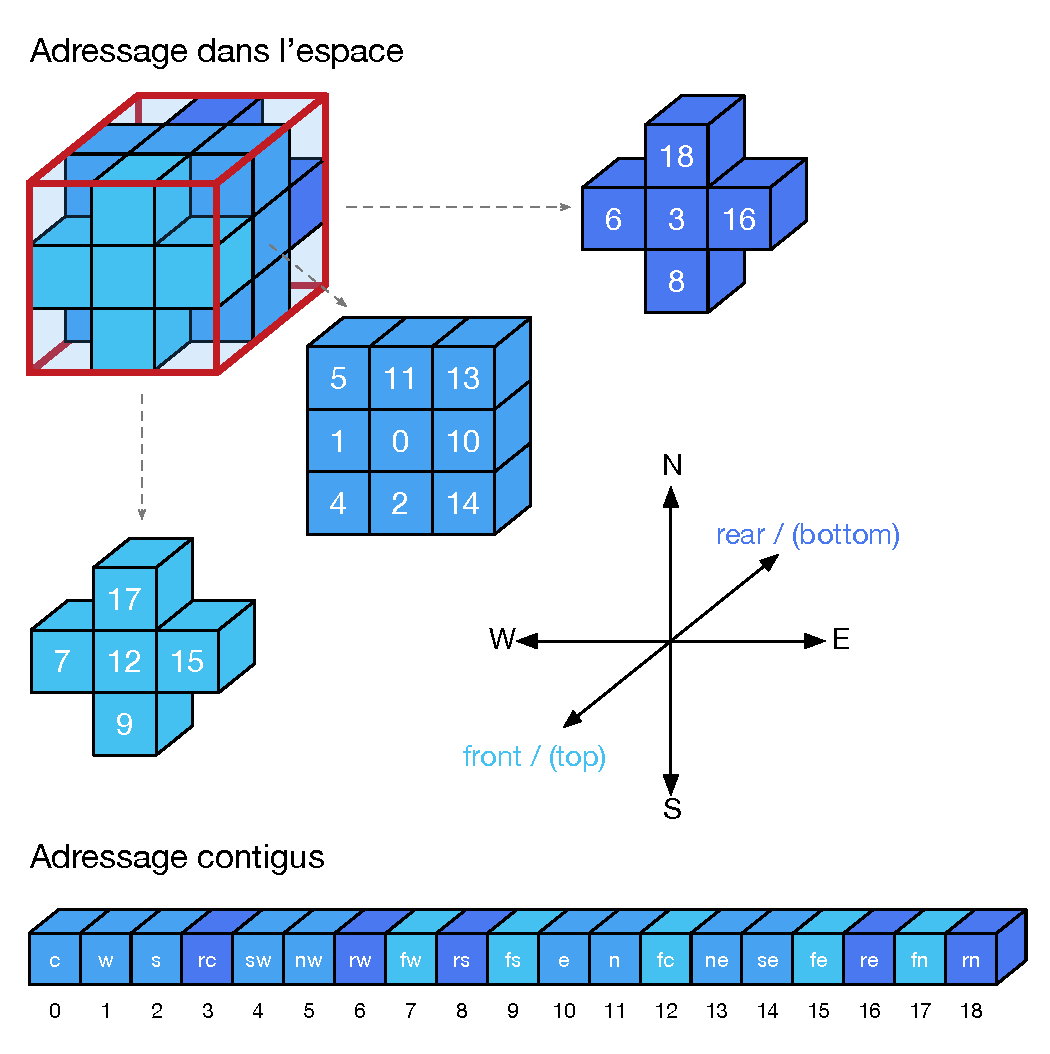
\includegraphics[scale=0.85, fbox]{images/index_population_palabos.pdf}
	\caption{Adressage d'une population sur Palabos}
	\label{fig:plb_population_index}
\end{figure}

La communication des populations entre le \acs{CPU} et le \acs{GPU} passe par la mémoire globale du \acs{GPU} à l'aide de la fonction \texttt{cudaMemcpy}. Ce type de transactions doit être réduit au minimum, car il s'agit du type d'accès mémoire le plus lent dans le contexte des \acs{GPU}. Hélas, Palabos requiert impérativement ces transactions à chaque itération, ce qui réduit les performances.

Toutefois, il n'est pas nécessaire de transférer l'intégralité du sous-domaine à chaque fois, à l'exception des cas suivants:
\begin{enumerate}
\item lors de la première itération, où il faut initialiser le sous-domaine avec les populations initiales depuis Palabos;
\item après une itération où l'on désire connaître l'état du domaine de recherche, où il faut rapatrier le sous-domaine.
\end{enumerate}

En effet, comme l'illustre la figure~\ref{fig:plb_enveloppes}, seules les communications de l'enveloppe extérieure et intérieure sont nécessaires.
L'enveloppe extérieure lors de l'envoi (de Palabos au \ac{CP}), pour permettre la propagation vers l'intérieur du sous-domaine lors du \ac{CS} et l'enveloppe intérieure lors de la réception (du \ac{CP} vers Palabos) pour mettre à jour les enveloppes extérieures des sous-domaines adjacents lors de la duplication des chevauchements (\textit{Duplicate overlaps}) en préparation de l'itération suivante. 

\begin{figure}[h]
	\centering
	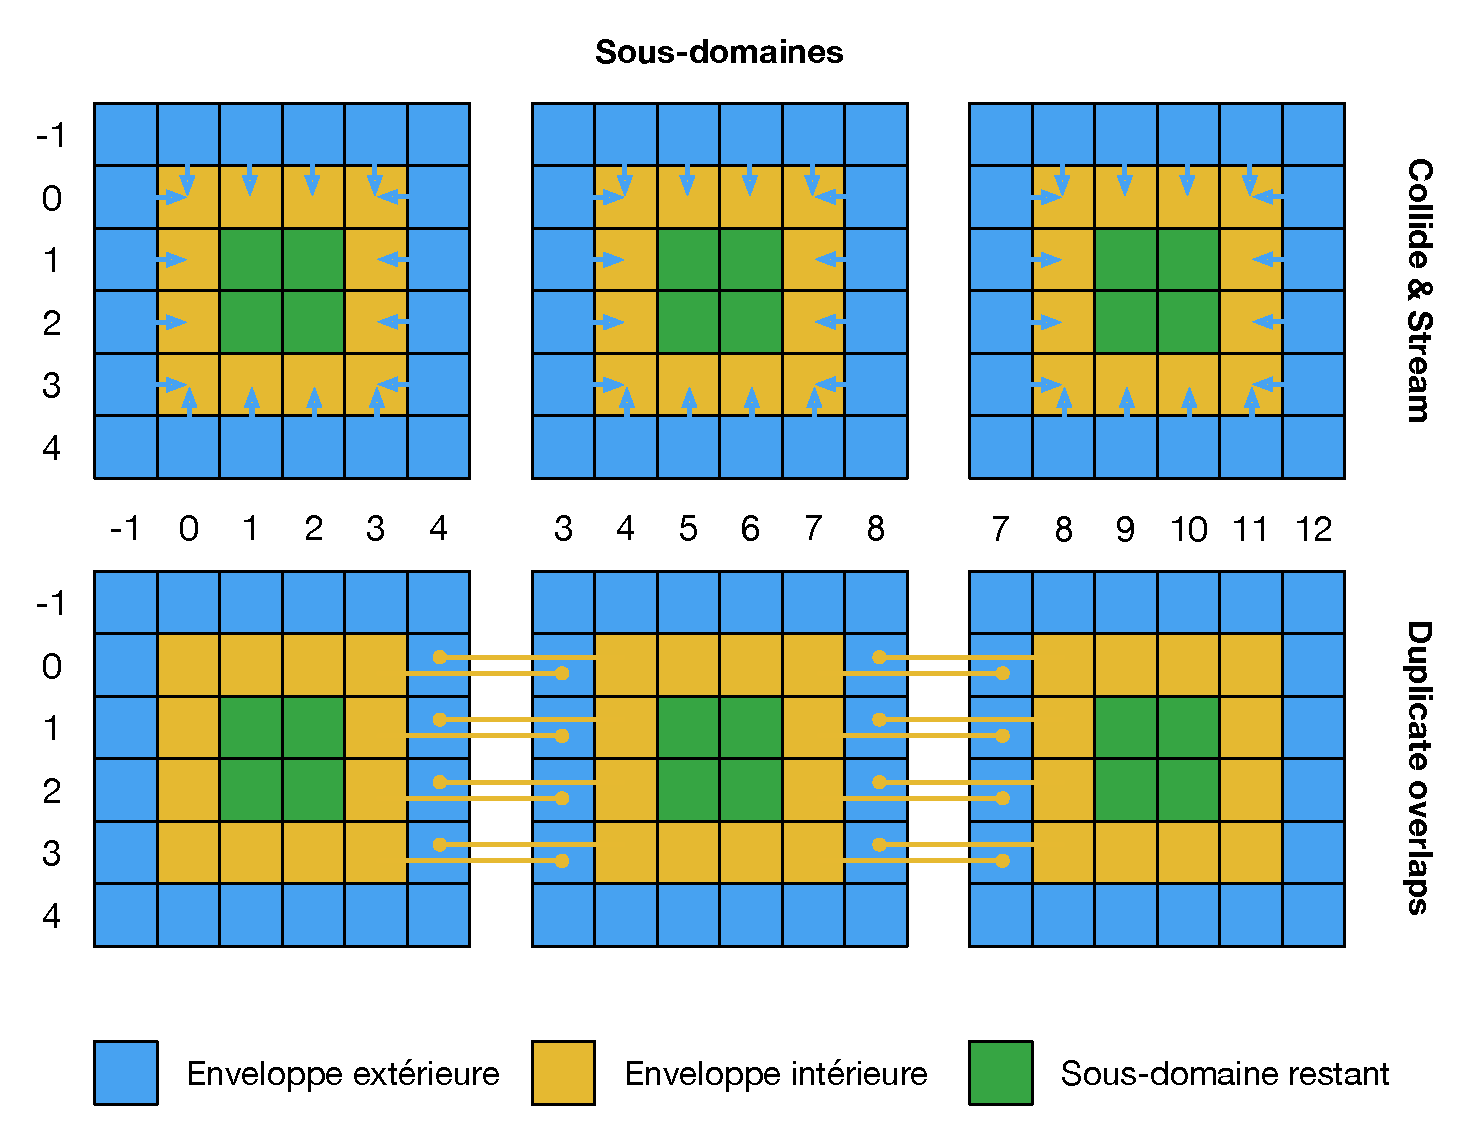
\includegraphics[scale=0.62, fbox]{images/enveloppes_interrieures_exeterrieures.pdf}
	\caption{Enveloppe extérieure et intérieure}
	\label{fig:plb_enveloppes}
\end{figure}

Un mécanisme est prévu par Palabos pour ne demander que le transfert de cette enveloppe. Lorsqu'il est utilisé, Palabos procède à un appel à \texttt{send} ou \texttt{receive} par face de l'enveloppe (figure~\ref{fig:plb_enveloppe_3d}), soit six appels. Bien que cela représente une multiplication par 6 du nombre d'appels (et par conséquent de l'overhead lié aux \texttt{cudaMemcpy}), cette méthode permet de réduire significativement l'espace mémoire à copier (figure~\ref{fig:plb_full_vs_partial_transfert}).

\begin{figure}[h]
	\centering
	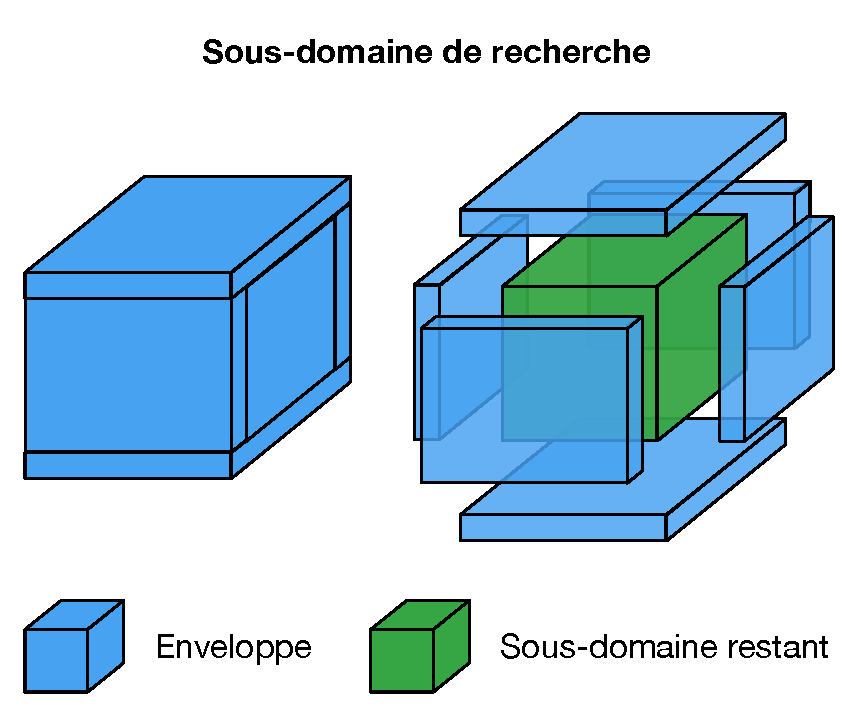
\includegraphics[scale=0.75, fbox]{images/enveloppe_3d_palabos.pdf}
	\caption{Enveloppe Palabos 3D}
	\label{fig:plb_enveloppe_3d}
\end{figure}

\begin{figure}[h]
	\centering
	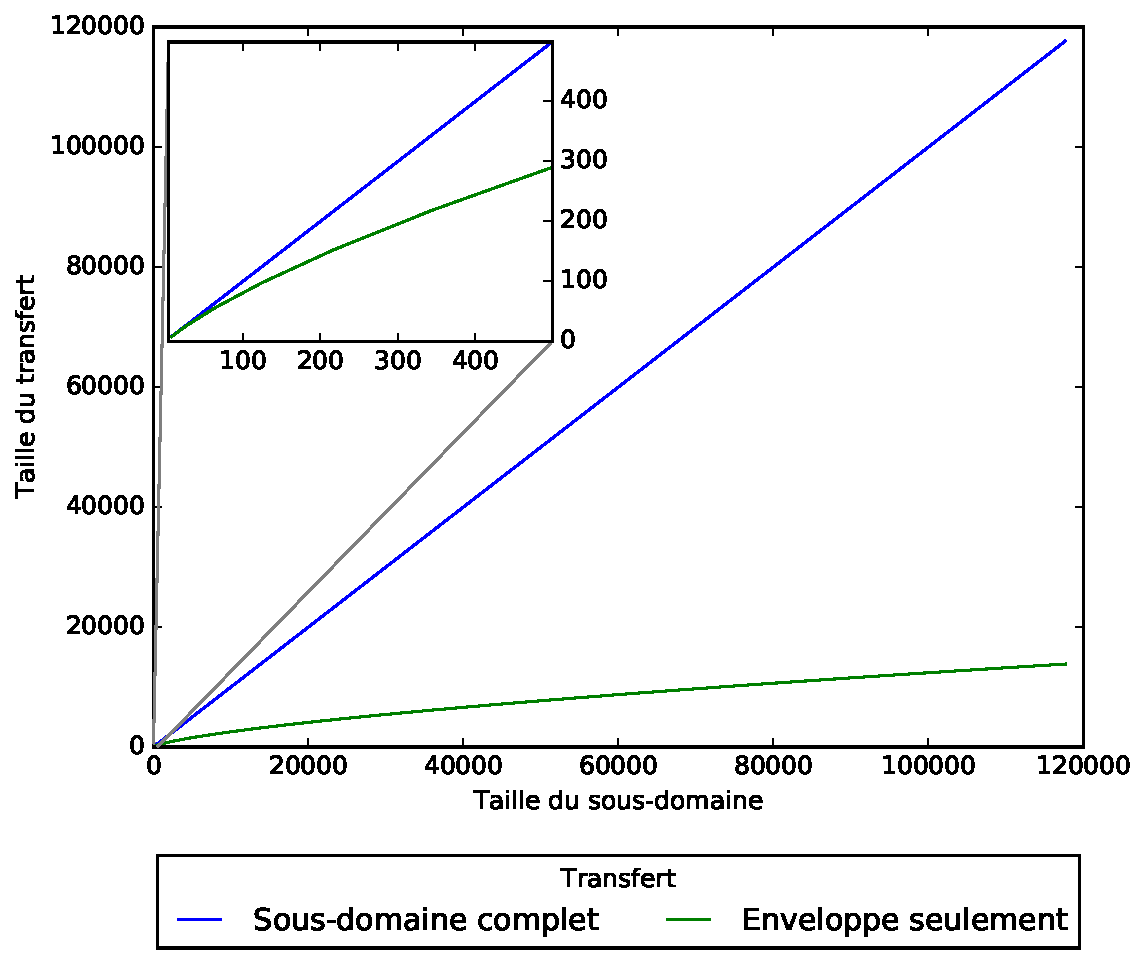
\includegraphics[scale=0.8, fbox]{../data/full_vs_partial_domain/full_vs_partial.pdf}
	\caption{Taille des transferts entre Palabos et un \ac{CP}}
	\label{fig:plb_full_vs_partial_transfert}
\end{figure}

\subsection{Stratégies de réorganisation des données}\label{title-strategie_reorganisation}
Comme le souligne la fin de la section~\ref{title-transfert_palabos_cp}, lorsque l'adressage des données est différent entre Palabos et le \ac{CP}, une étape de réorganisation doit intervenir lors du processus de transfert. Dans le cas présent, Palabos utilise l'arrangement mémoire \acs{AoS}, tandis que l'implémentation \acs{GPU} utilise l'arrangement \acs{SoA}.

Deux stratégies de réorganisation ont été explorées:
\begin{enumerate}
\item \textbf{Réorganisation sur \acs{CPU} et transfert}: Cette stratégie réarrange les données reçues ou à transférer sur le \acs{CPU} dans l'ordre qu'utilise le \acs{GPU} en mémoire globale et tente de profiter de la forme du sous-domaine transmis pour réduire le nombre d'appels à \texttt{cudaMemcpy} lorsque la mémoire est contiguë.

L'ordre dans lequel la réorganisation et le transfert ont lieu dépend de l'opération:
\begin{itemize}
\item \texttt{send}:
\begin{enumerate}
\item réorganisation mémoire sur \acs{CPU};
\item transfert mémoire du \acs{CPU} au \acs{GPU}
\end{enumerate}
\item \texttt{receive}:
\begin{enumerate}
	\item transfert mémoire du \acs{GPU} au \acs{CPU}
	\item réorganisation mémoire sur \acs{CPU};
\end{enumerate}
\end{itemize}

Un transfert de l'ensemble du sous-domaine est simplement réalisé par 19 \texttt{cudaMemcpy} (un par tableau). Toutefois, il est impossible d'utiliser cette méthode telle quelle lors d'un transfert partiel (pour une partie de l'enveloppe par exemple). En effet, comme l'illustre la figure~\ref{fig:adressage_cp}, certaines faces ont un adressage contigu, tandis que d'autres non.

L'étape de transfert tire parti des faces dont l'adressage est contigu pour réduire le nombre d'appels à \texttt{cudaMemcpy}. Par conséquent, voilà comment seraient transférées les faces suivantes:
\begin{itemize}
\item $XZ$: un \texttt{cudaMemcpy} pour l'ensemble de la face et par direction (soit 19);
\item $XY$: un \texttt{cudaMemcpy} par ligne et par direction (soit $4\times19 = 76$);
\item $YZ$: un \texttt{cudaMemcpy} par population et par direction (soit $4\times4\times19 = 304$);
\end{itemize}

On constate que le nombre de \texttt{cudaMemcpy} devient très important sur les faces dont les indices ne sont pas consécutifs. De plus, ils ne transfèrent qu'une seule valeur à la fois. Une telle face, d'un domaine $100\time100\times100$, nécessite 190000 appels à \texttt{cudaMemcpy} pour être transférée. 
Cette stratégie offre par conséquent de très mauvaises performances.

\item \textbf{Transfert et réorganisation sur \acs{GPU}}: Plutôt que réorganiser les données sur le \acs{CPU}, cette stratégie utilise à cette fin le \acs{GPU} et transfère d'un seul bloc les données entre le \acs{CPU} et le \acs{GPU} avec un unique \texttt{cudaMemcpy}. Là encore, l'opération dicte l'ordre dans lequel la réorganisation et le transfert à lieu ont lieu:
\begin{itemize}
	\item \texttt{send}:
	\begin{enumerate}
		\item transfert mémoire du \acs{CPU} au \acs{GPU}
		\item réorganisation mémoire sur \acs{GPU};
	\end{enumerate}
	\item \texttt{receive}:
	\begin{enumerate}
		\item réorganisation mémoire sur \acs{GPU};
		\item transfert mémoire du \acs{GPU} au \acs{CPU}
	\end{enumerate}
\end{itemize}
\end{enumerate}

On observe une inversion de l'ordre des opérations, par rapport à la stratégie précédente. Dans le cas du \texttt{send}, les données sont directement transférées au \acs{GPU}, puis exécutent un \textit{kernel} dédié à la réorganisation et la copie des données vers la structure de donnée utilisées par le \textit{kernel} de calcul.

Dans le cas du \textit{receive}, un autre \textit{kernel}, dédié cette fois à la réorganisation et la copie des données depuis la structure de donnée de calcul, est exécuté avant que les donnés soient finalement transférés du \acs{GPU} au \acs{CPU}.

Cette méthode réduit à la fois considérablement le nombre d'appels à \texttt{cudaMemcpy} et profite de capacité de parallélisation du \acs{GPU} pour accélérer la réorganisation des données. Elle présente ainsi de bien meilleures performances.

\begin{figure}[h]
	\centering
	\subfigure[Face $YZ$ avant (x=0)]{%
		\centering
		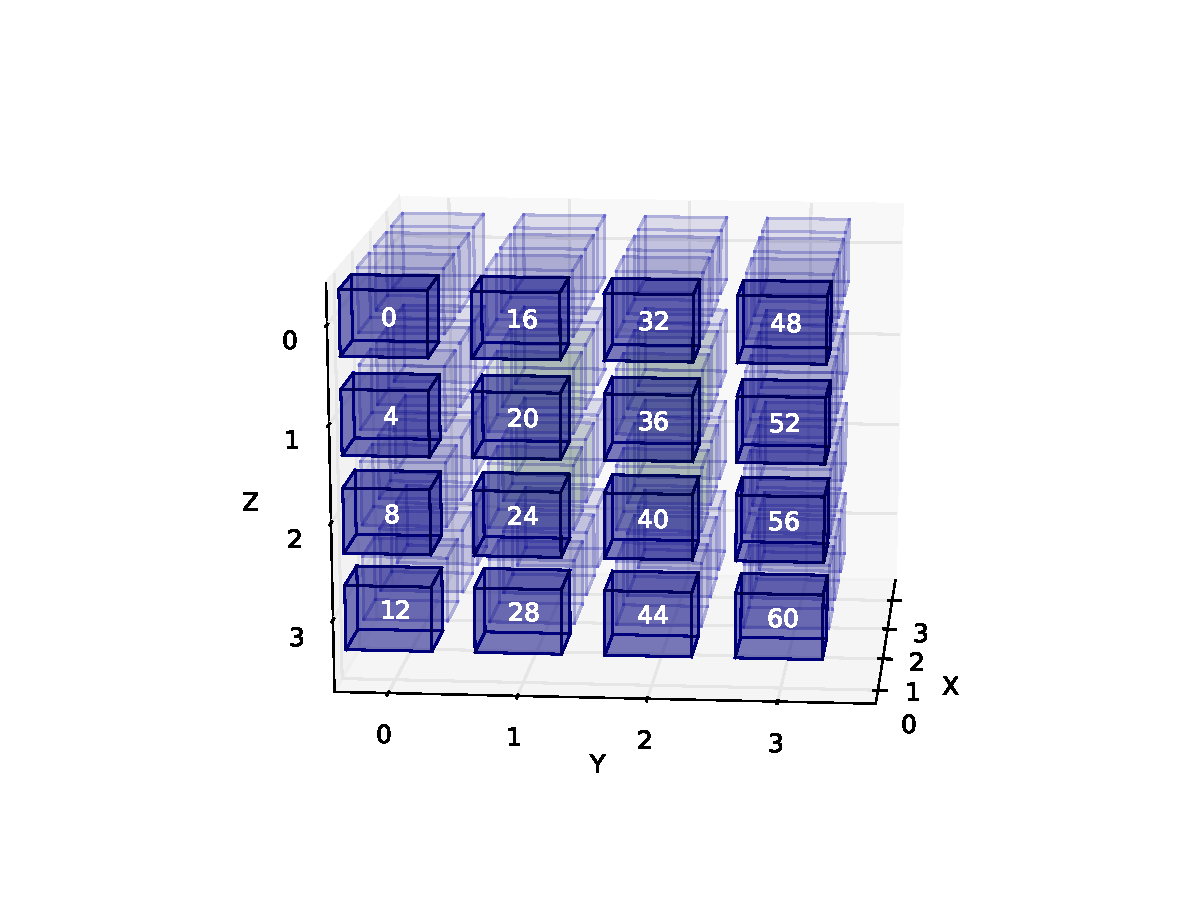
\includegraphics[fbox, scale=0.6, trim=115 50 110 60, clip]{images/cp_index_x_0.pdf}
		\label{fig:cp_index_x_0}
	}
	\subfigure[Face $YZ$ arrière (x=3)]{%
		\centering
		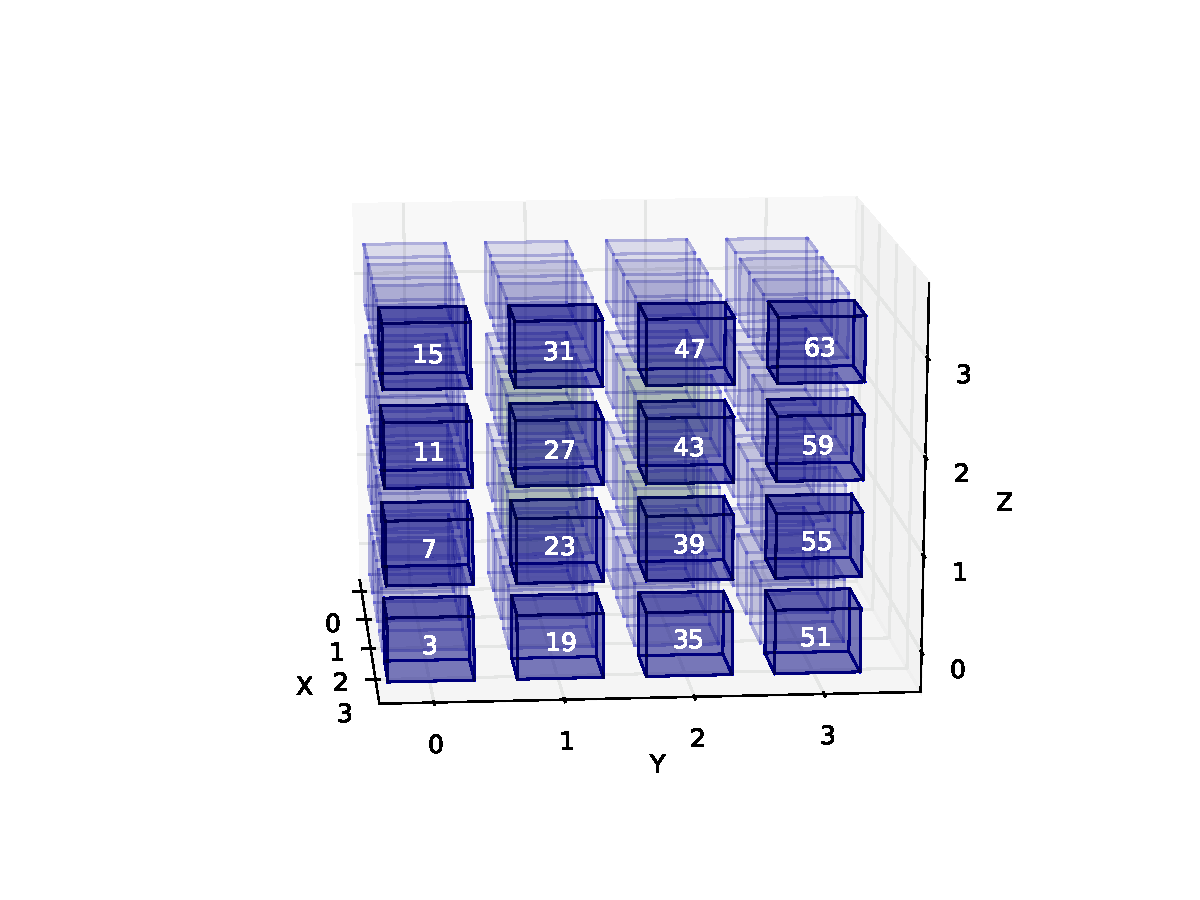
\includegraphics[fbox, scale=0.6, trim=140 50 90 60, clip]{images/cp_index_x_3.pdf}
		\label{fig:cp_index_x_3}
	}
	\subfigure[Face $XZ$ avant (y=0)]{%
	\centering
	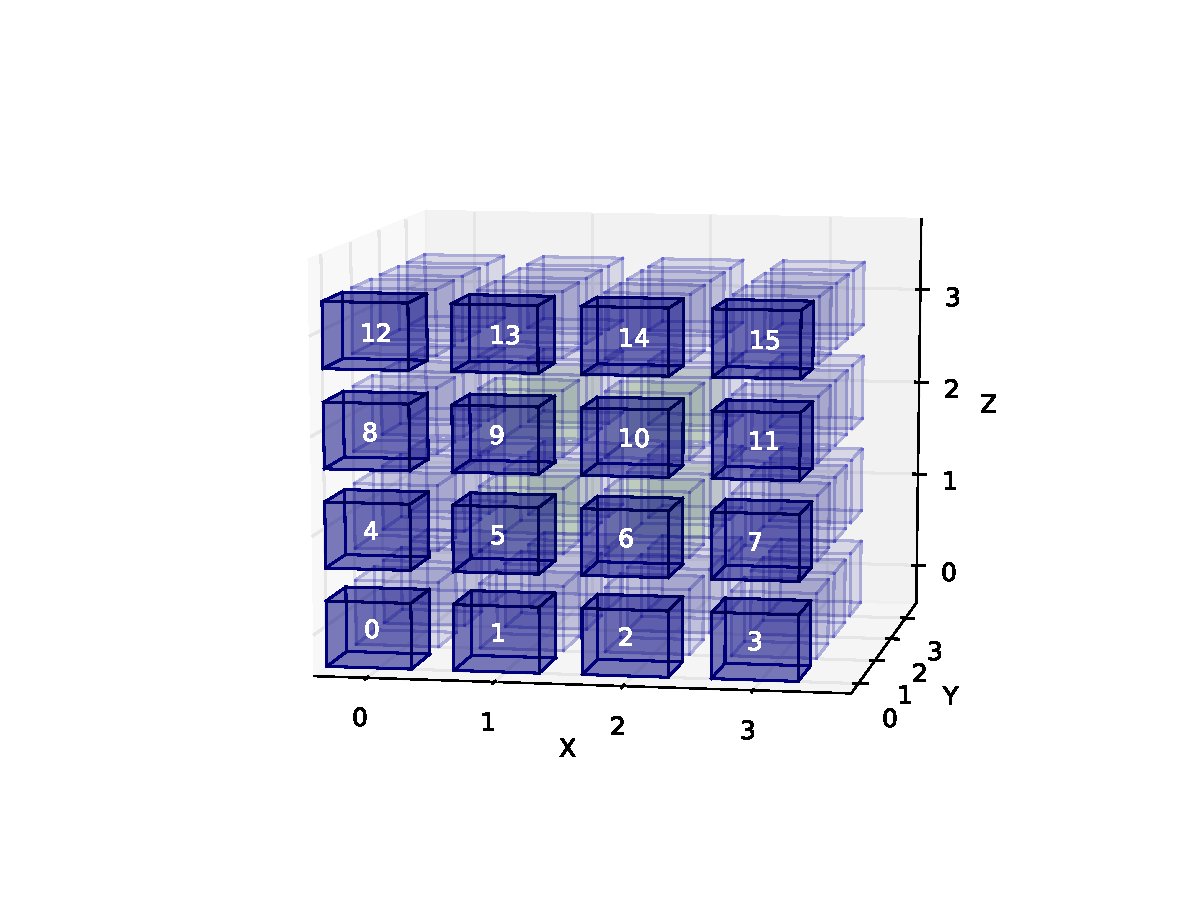
\includegraphics[fbox, scale=0.6, trim=130 50 90 60, clip]{images/cp_index_y_0.pdf}
	\label{fig:cp_index_y_0}
	}
	\subfigure[Face $XZ$ arrière (y=3)]{%
		\centering
		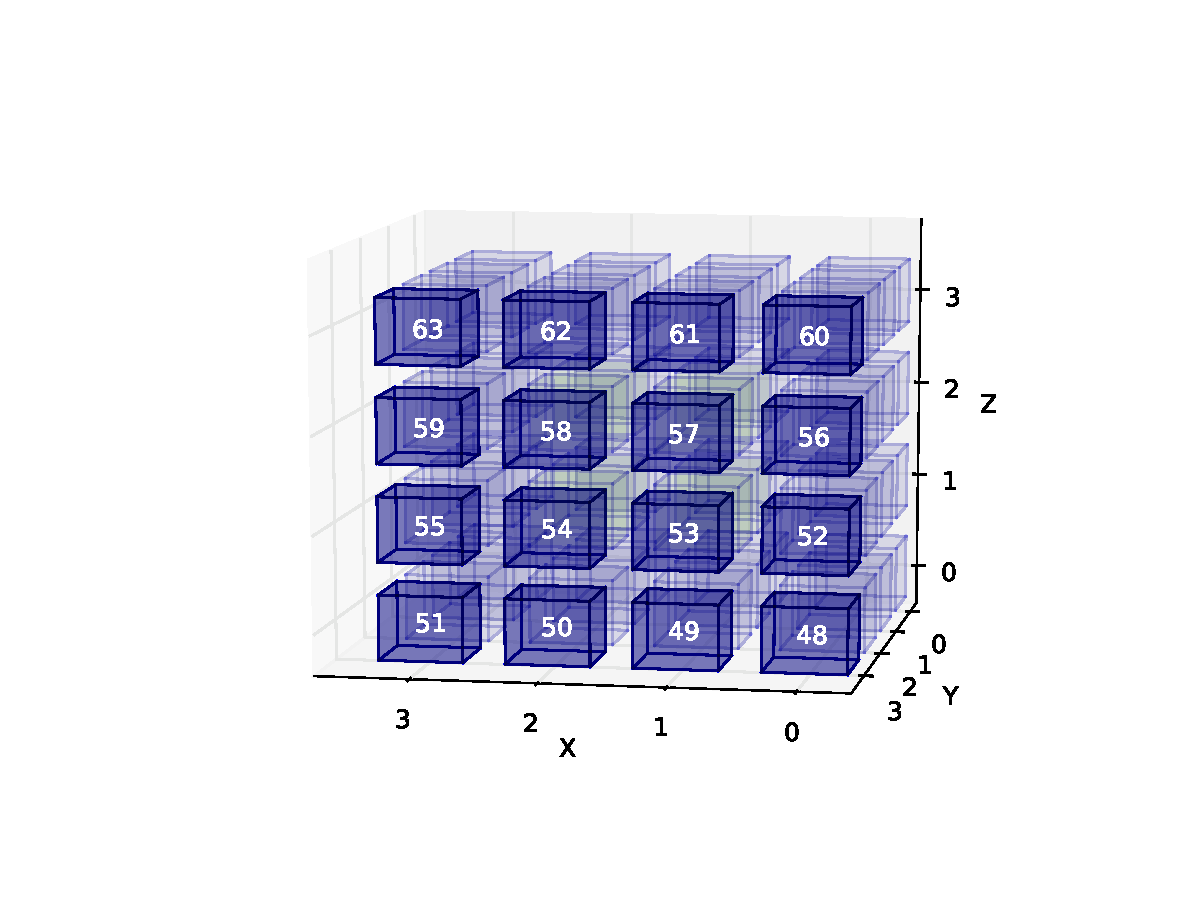
\includegraphics[fbox, scale=0.6, trim=130 50 90 60, clip]{images/cp_index_y_3.pdf}
		\label{fig:cp_index_y_3}
	}
		\subfigure[Face $XY$ avant (z=0)]{%
		\centering
		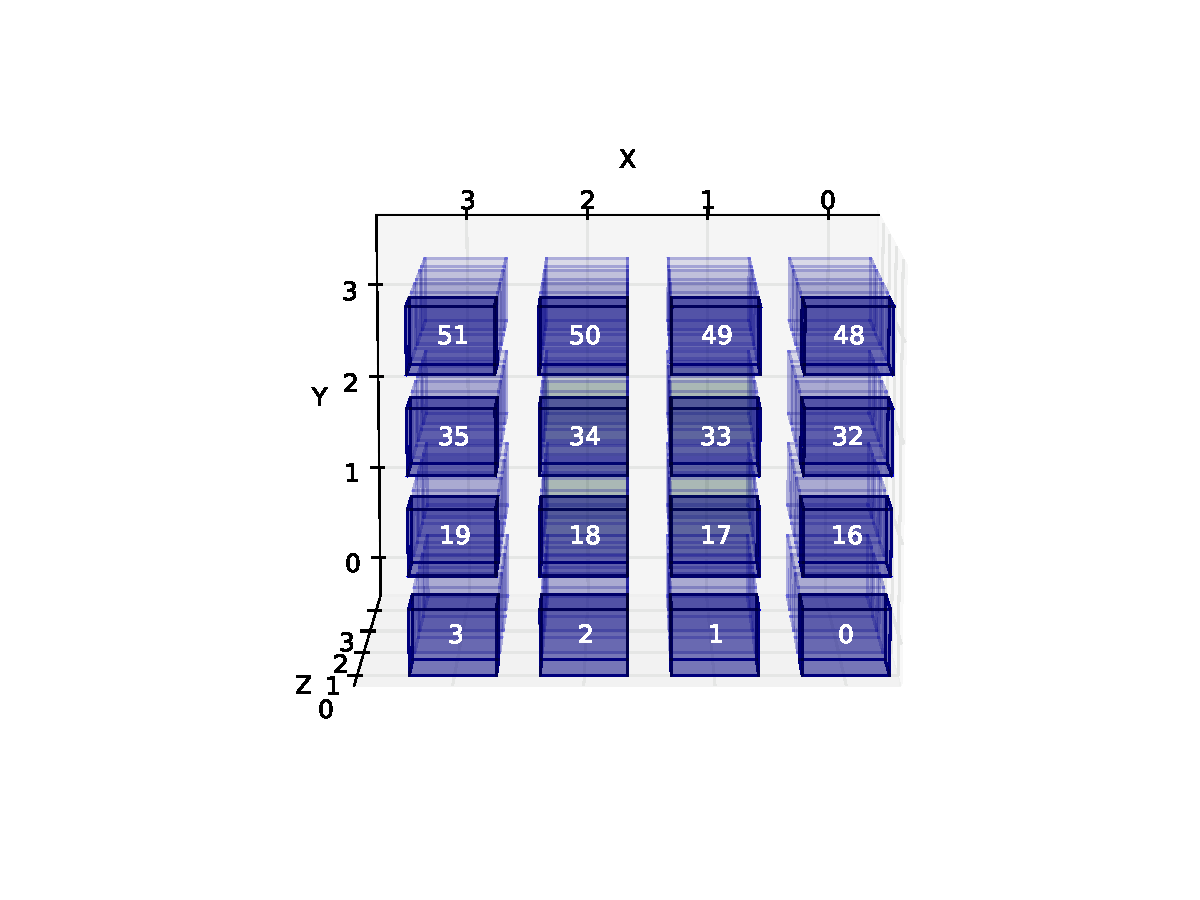
\includegraphics[fbox, scale=0.6, trim=130 70 90 60, clip]{images/cp_index_z_0.pdf}
		\label{fig:cp_index_z_0}
	}
	\subfigure[Face $XY$ arrière (z=3)]{%
		\centering
		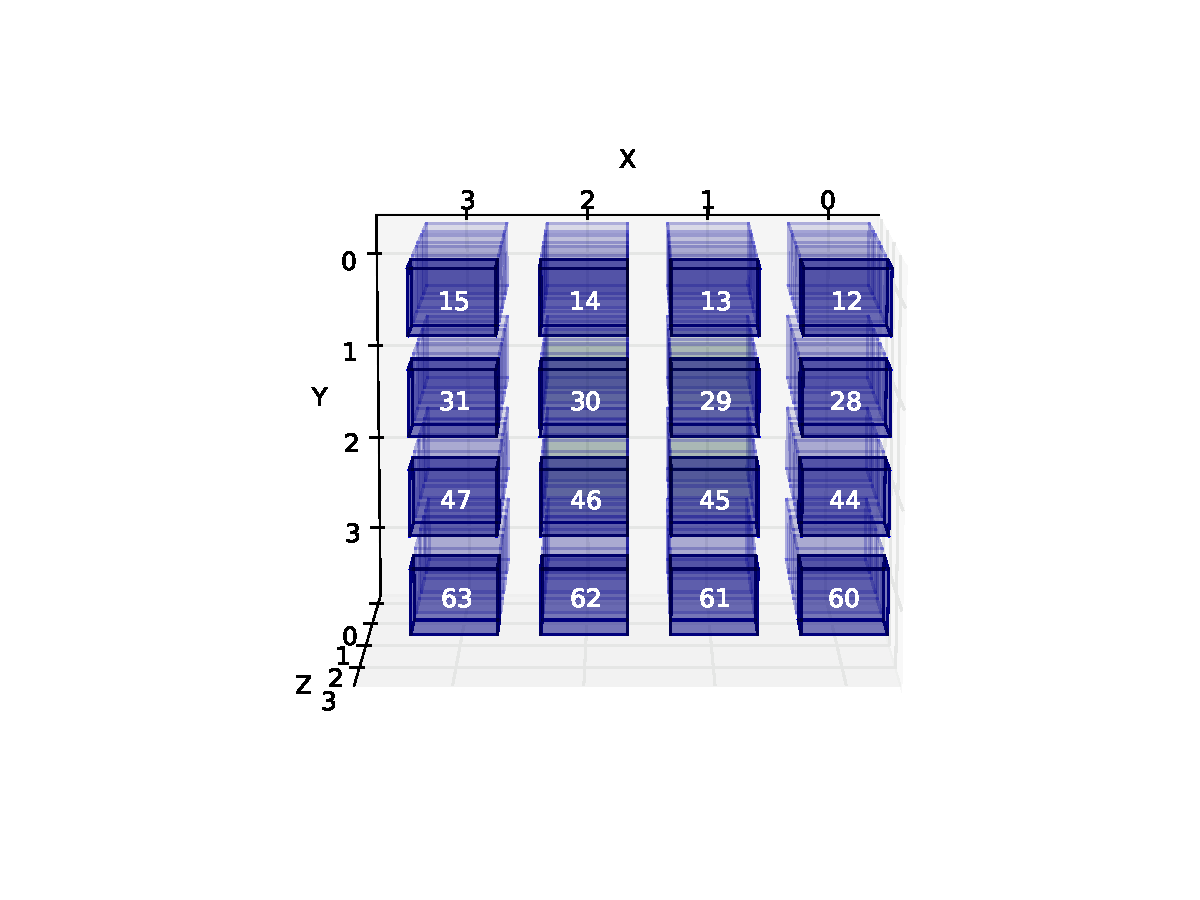
\includegraphics[fbox, scale=0.6, trim=130 70 90 60, clip]{images/cp_index_z_3.pdf}
		\label{fig:cp_index_z_3}
	}
	\caption{Adressage des populations dans un sous-domaine $4\times4$}
	\label{fig:adressage_cp}
\end{figure}

\subsection{Simulation d'écoulement dans une cavité} \label{title-cavity_benchmark}
Pour tester l'intégration à Palabos et en mesurer les performances, l'implémentation \texttt{cavity\_benchmark} a été réalisée. À l'exception de quelques modifications (destinées à rendre les exécutions configurables notamment), leur code est essentiellement copié de l'exemple \texttt{coProcessor} fournit par Palabos.

Cette implémentation simule l'écoulement d'un fluide dans une cavité. Le domaine est cubique et découpé en vingt-sept sous-domaines. Il est possible de choisir les dimensions du domaine central. Les autres domaines ajustent alors les leurs automatiquement. La figure~\ref{fig:decoupage_sous_domaine_cavity_benchmark} illustre le découpage et dimensionnement des sous-domaines pour deux exemples. Le premier pour un sous-domaine central dont les côtés mesurent le $\nicefrac{1}{3}$ de ceux du domaine et  $\nicefrac{2}{3}$ pour le second.

\begin{figure}[H]
	\centering
	\subfigure[3500 itérations]{%
		\centering
		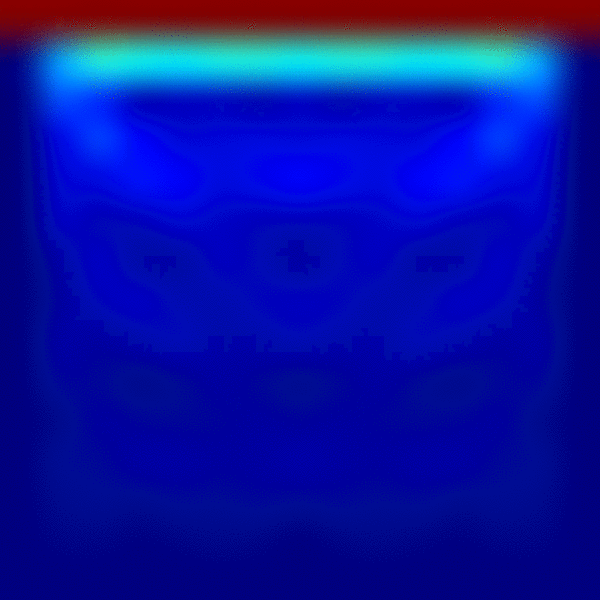
\includegraphics[fbox, scale=0.3]{images/cavity_benchmark/uNorm003500.png}
		\label{fig:cavity_benchmark3500}
	}
	\subfigure[42000 itérations]{%
		\centering
		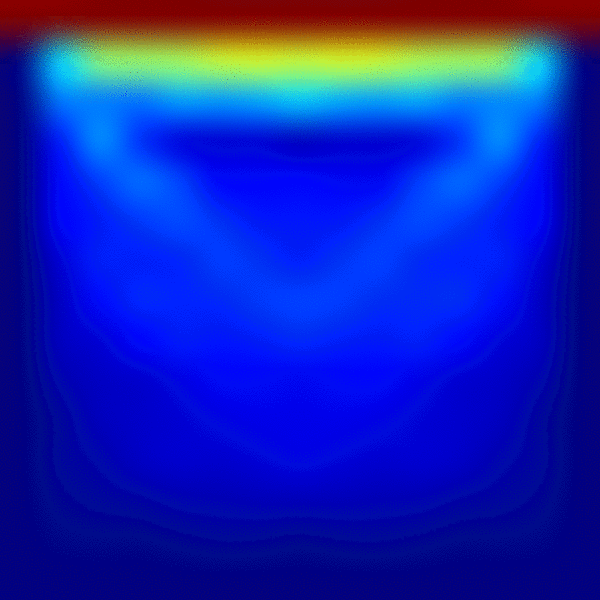
\includegraphics[fbox, scale=0.3]{images/cavity_benchmark/uNorm042000.png}
		\label{fig:cavity_benchmark42000}
	}
	\caption{Images générées par \texttt{cavity\_benchmark} d'un écoulement dans une cavité}
	\label{fig:cavity_benchmark}
\end{figure}

\begin{figure}[H]
	\centering
	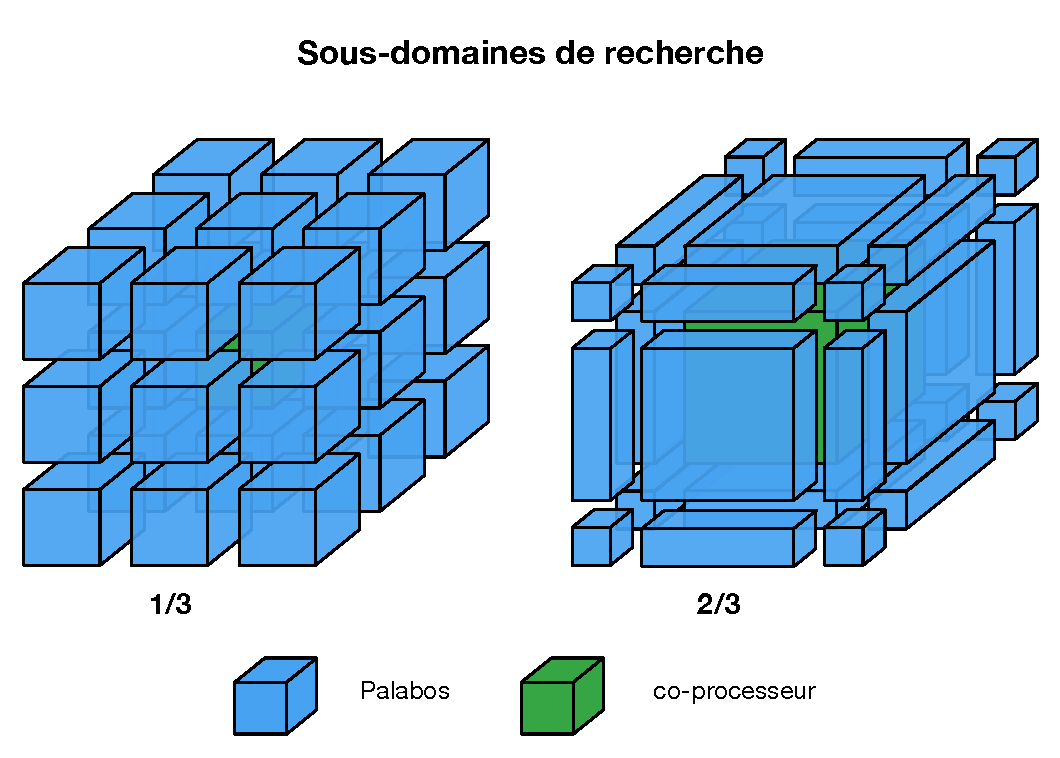
\includegraphics[scale=0.65, fbox]{images/decoupage_sous_domaine_cavity_benchmark.pdf}
	\caption{Dimensionnement des sous-domaines de \texttt{cavity\_benchmark}}
	\label{fig:decoupage_sous_domaine_cavity_benchmark}
\end{figure}

Le sous-domaine central est confié au co-processeur \acs{GPU} (ou à un co-processeur \acs{CPU} à des fins de test si on le désire) tandis que les vingt-six autres qui l'entourent sont calculés sur le \acs{CPU} par Palabos.

